%Chapter 5 - Current state of the MEGA65 project
%What is the current state of the MEGA65 project?

\chapter{Current state of the MEGA65 project as of March, 2019}
\label{cha: Chapter5}
This chapter discusses the current state of the MEGA65 project in both its form-factors: the MEGAphone hand-held console . 
%----------------------------------------------------------------------------------------
%----------------------------------------------------------------------------------------
\section{FPGA based architecture}
The core of both form-factors of the MEGA65 is the FPGA-based components, such as the CPU and video controller, designed by Dr. Paul Gardner-Stephens. The FPGA components are practically complete, with Detlef suggesting a 99\% compatibility with Commodore 64 software. Achieving the last 1\% may be as hard as achieving the previous 99\% though, as such it may not be worth the time to achieve full 100\% compatibility. There are still some bugs present in the FPGA components which need addressed.

\section{Software}

\subsection{Operating System}

\subsection{BIOS/firmware}

\subsection{Applications}



\section{MEGAphone}
This section looks at the current state of the MEGAphone. The MEGAphone is the hand-held console form-factor of the MEGA65. 

\subsection{Hardware}
The MEGAphone electronics hardware is currently in an alpha stage, the PCB is in its first revision and is mostly populated with components but there is expected to be faults in the design. A picture of the PCB with and without components is shown below in figure \ref{MEGAphone_PCB_r1_empty} and \ref{MEGAphone_PCB_r1_populated}. A visual inspection of the PCB and discussion with Dr Paul Gardner-Stephens led to the following lists of faults, things to be tested and other note-worthy decisions relating to the current state of the MEGAphone hardware. \\

\begin{figure} \begin{center}
\includegraphics[width=.3\linewidth]{pics/MEGAphone_PCB_r1_empty_front} 
\includegraphics[width=.3\linewidth]{pics/MEGAphone_PCB_r1_empty_back} 
\end{center} 
\caption{MEGAphone PCB Revision 1 from the front and back when not populated with components. Front side is shown of the left.\\}
\label{MEGAphone_PCB_r1_empty}
\end{figure}

\begin{figure} \begin{center}
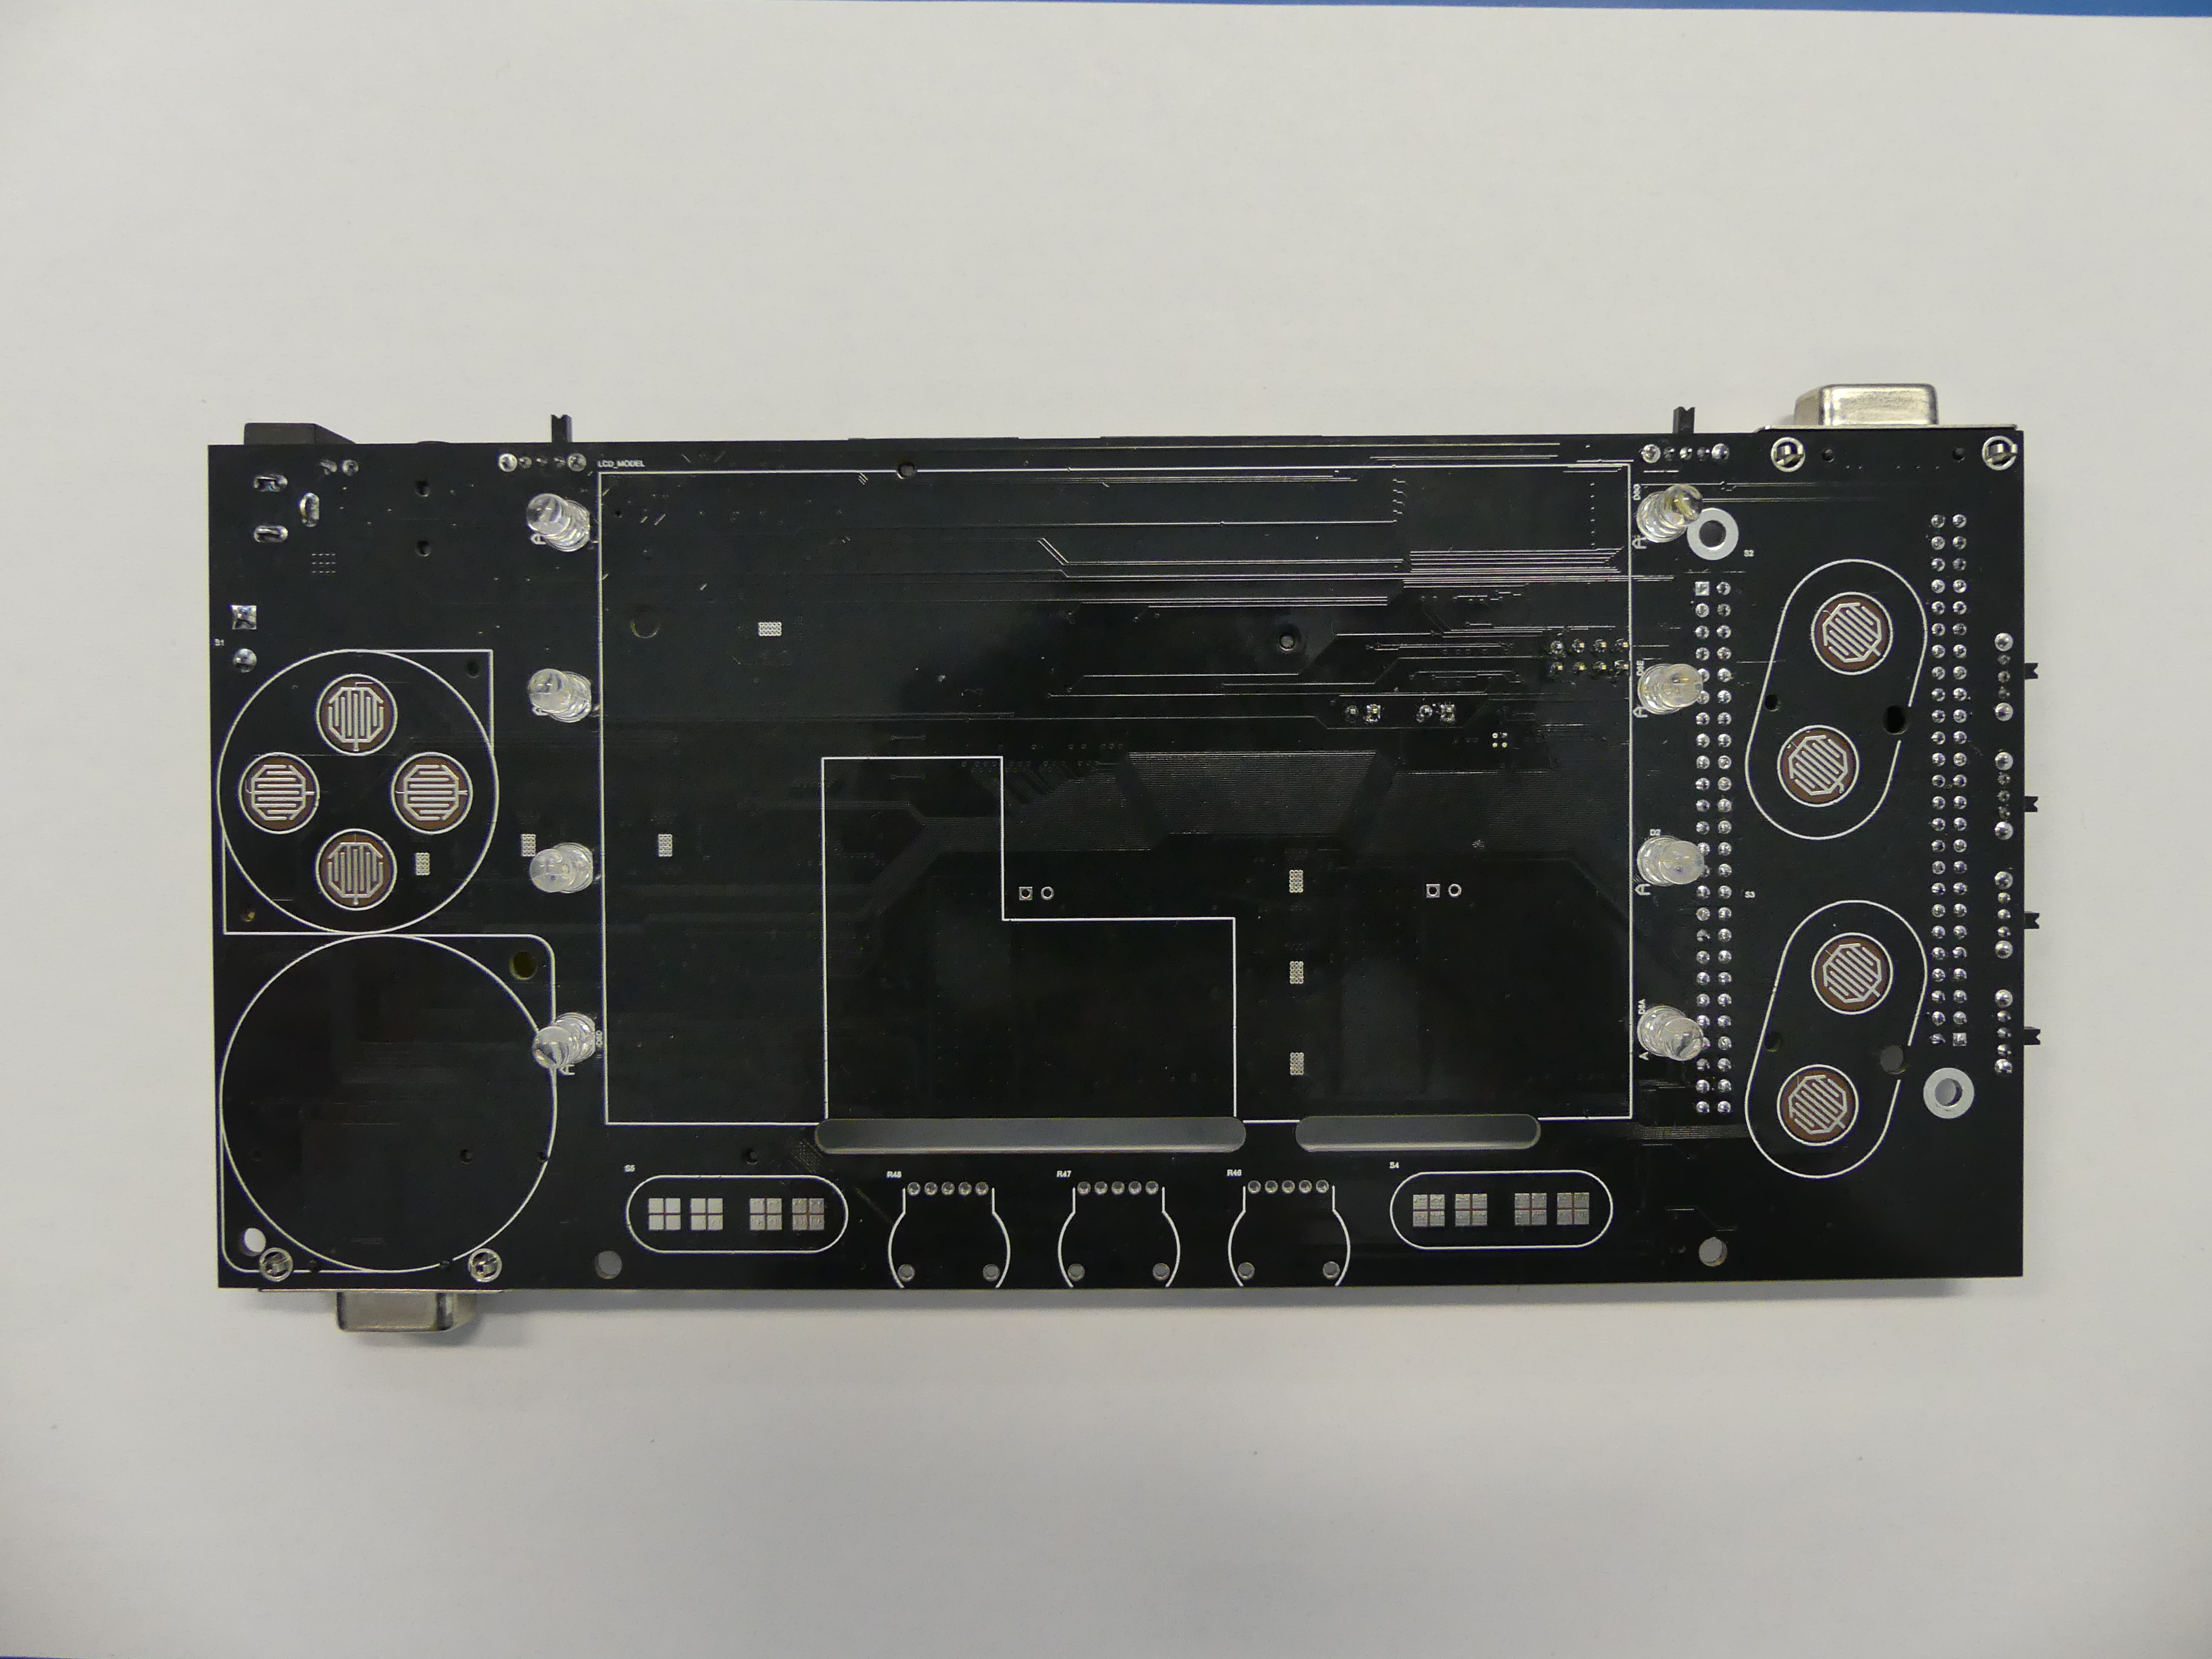
\includegraphics[width=.3\linewidth]{pics/MEGAphone_PCB_r1_populated_front} 
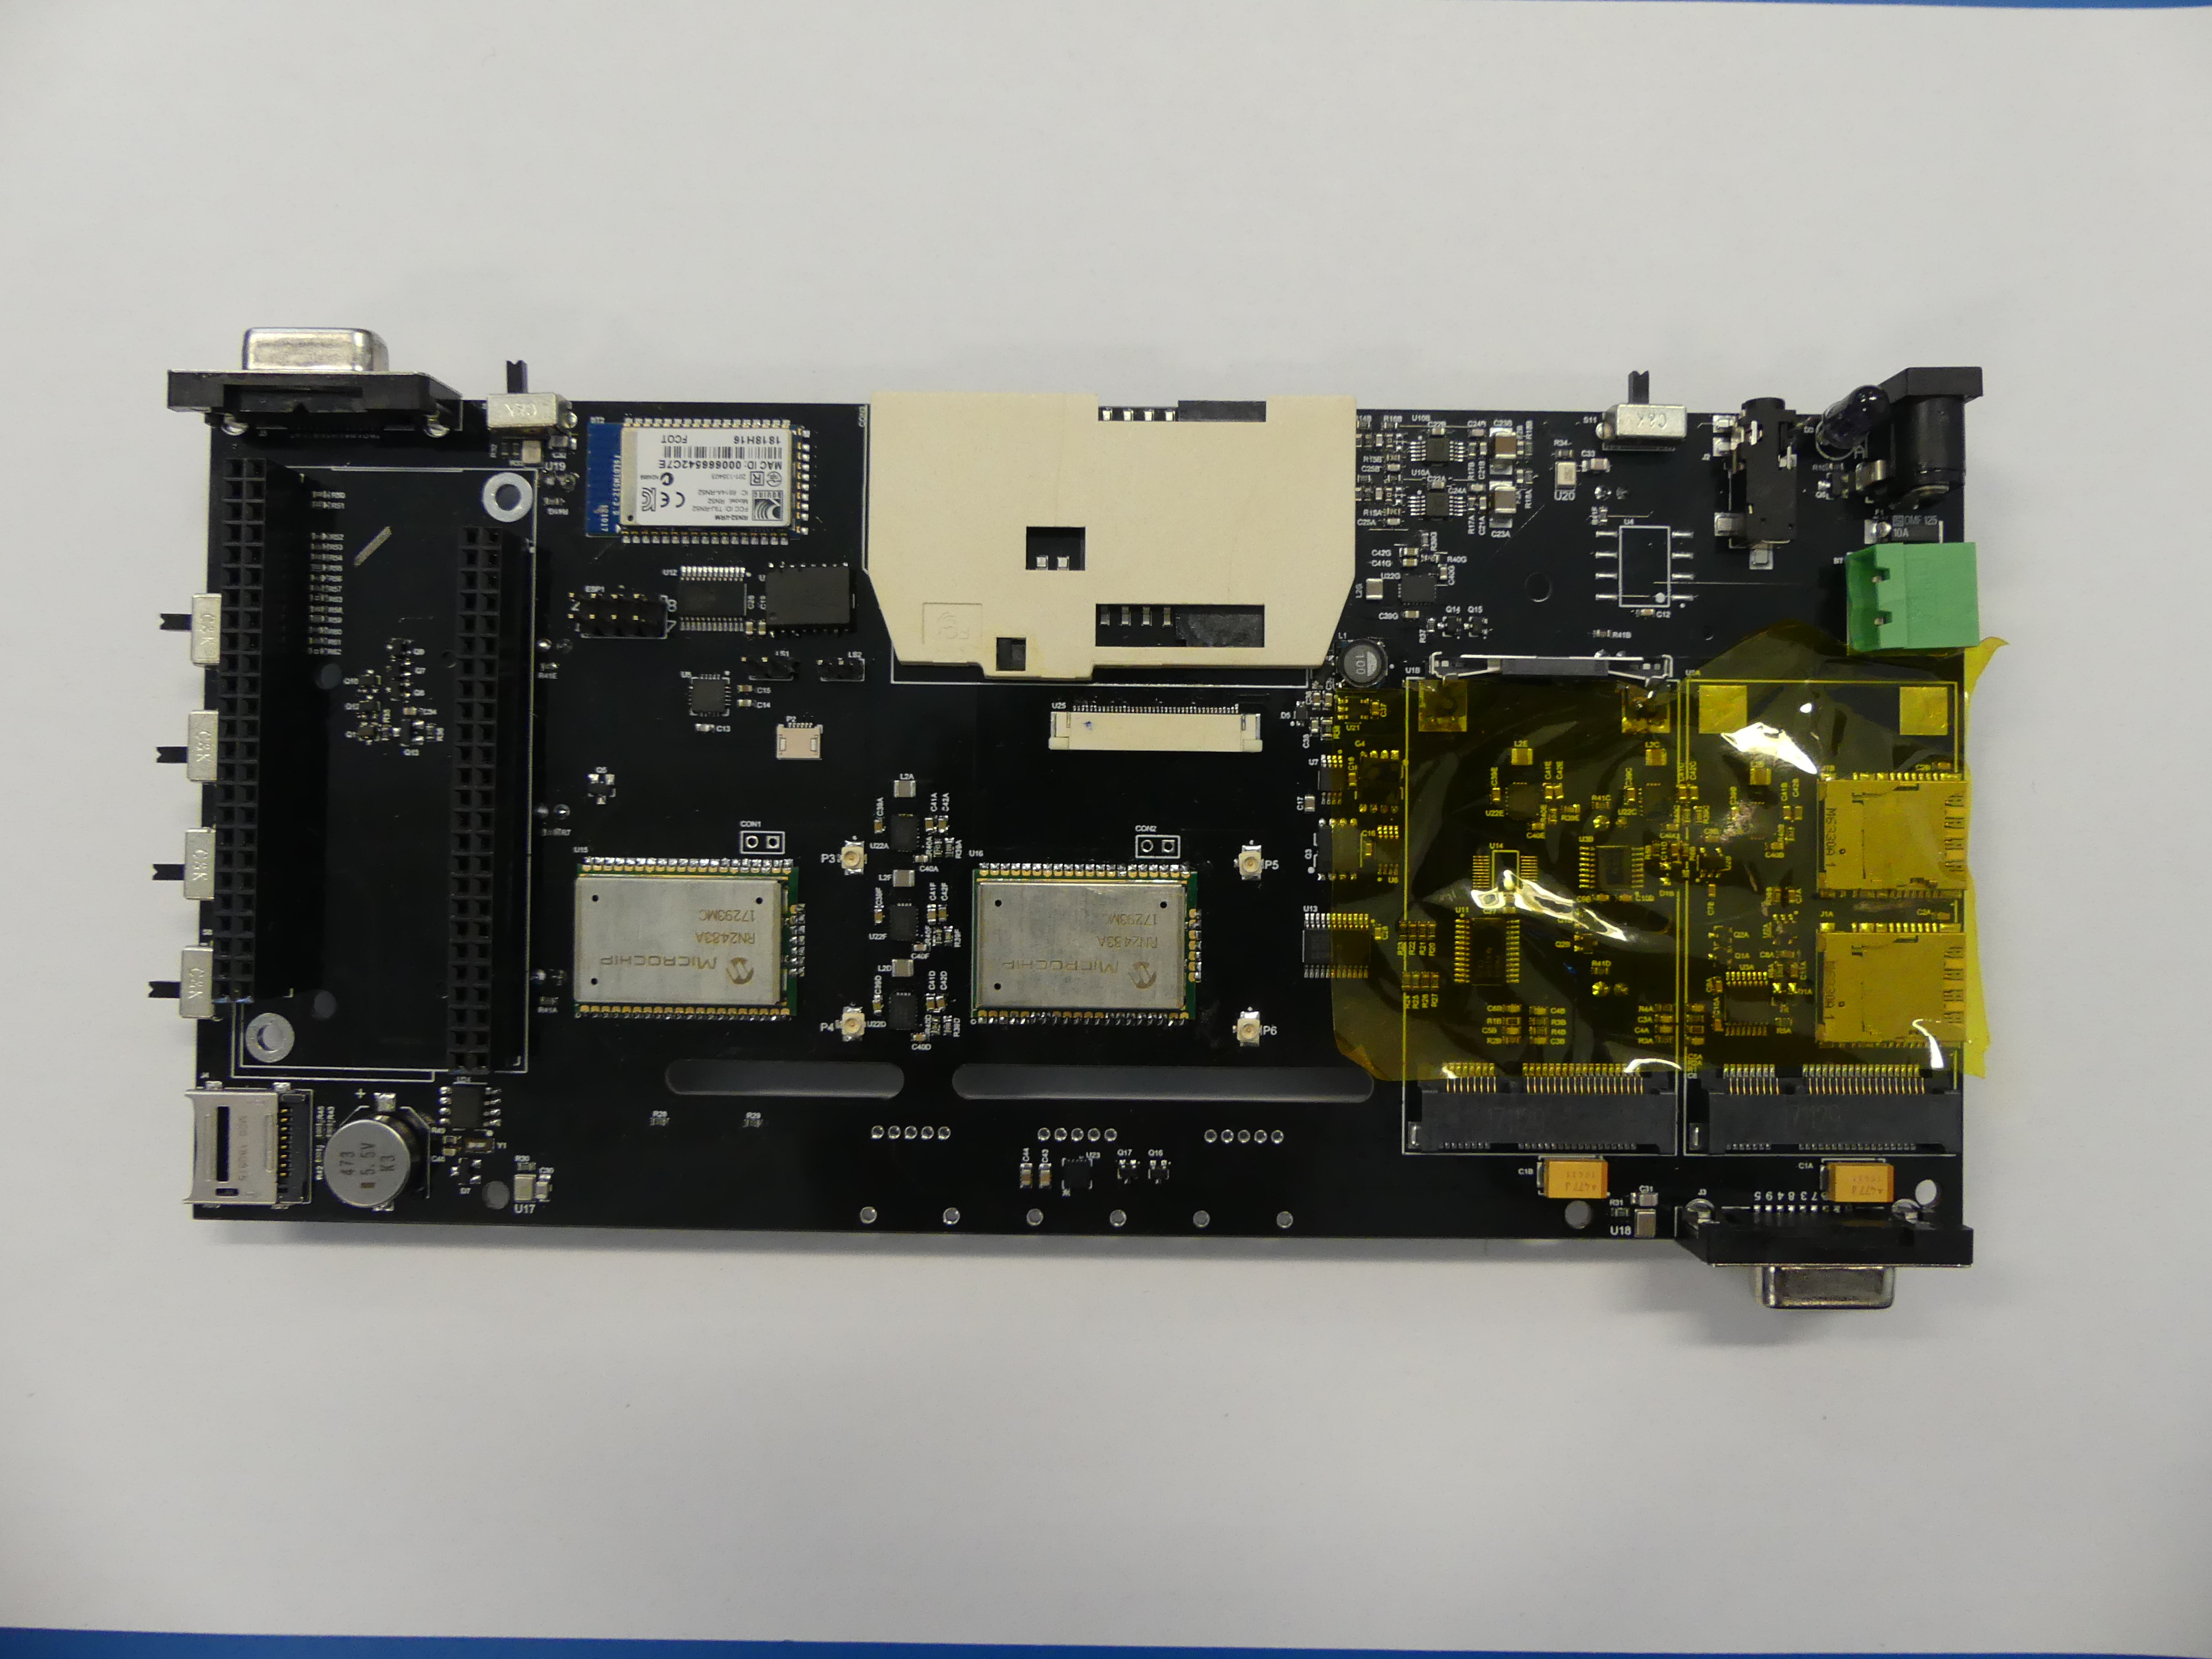
\includegraphics[width=.3\linewidth]{pics/MEGAphone_PCB_r1_populated_back} 
\end{center} 
\caption{MEGAphone PCB Revision 1 from the front and back populated with components. Front side is shown of the left.\\}
\label{MEGAphone_PCB_r1_populated}
\end{figure}


\textbf{Faults in Hardware}
\begin{enumerate}
\item The joystick connector, J3, is the wrong gender, currently it is female where as it should be male, figure \ref{MEGAphone_PCB_r1_J3}.
\item U1A and U1B, the footprint of the latch that holds the cellular modem is in the wrong position, figure \ref{MEGAphone_PCB_r1_U1A}.
\item U14 is not populated, this is the external joystick controller, figure \ref{MEGAphone_PCB_r1_U14}. 
\item U4 is currently missing, this is the Analogue-to-Digital converter for the microphone, figure \ref{MEGAphone_PCB_r1_U4}.
\item U25 needs to be moved a few millimetres to the right (when looking at the PCB face the component is mounted to) and also a couple of millimetres towards the slot which the ribbon runs through. This is to allow the ribbon cable to connect easier, figure \ref{MEGAphone_PCB_r1_U25}.
\item P2 need to be re-positioned a couple of millimetres towards the ribbon cable slot to allow the ribbon to connect easier \ref{MEGAphone_PCB_r1_P2}.
\item U15 may need to be moved a few millimetres to the left (when looking at the component) to allow for the ribbon cable to reach P2 without rubbing on U15 figure \ref{MEGAphone_PCB_r1_P2}.
\item LED power indicator are slightly too close together to allow the screen cover to fit between them \ref{MEGAphone_PCB_r1_LED}.
\item U9 which is the SPI flash chip, the footprint is wrong i.e. doesn't match the part, figure \ref{MEGAphone_PCB_r1_U9}.
\item R46, R47 and R48, the thumb wheels for volume control, are missing and currently on back order, figure \ref{MEGAphone_PCB_r1_R49_R48_R47}.
\item Found the PCB is outputting over 6.45 Volts where it should be outputting 3.3V. \\
\end{enumerate}

\begin{figure} \begin{center}
\includegraphics[width=.3\linewidth]{pics/MEGAphone_PCB_r1_J3} 
\end{center} 
\caption{Close up of Joystick connector J3, which should be a male connector.\\}
\label{MEGAphone_PCB_r1_J3}
\end{figure}

\begin{figure} \begin{center}
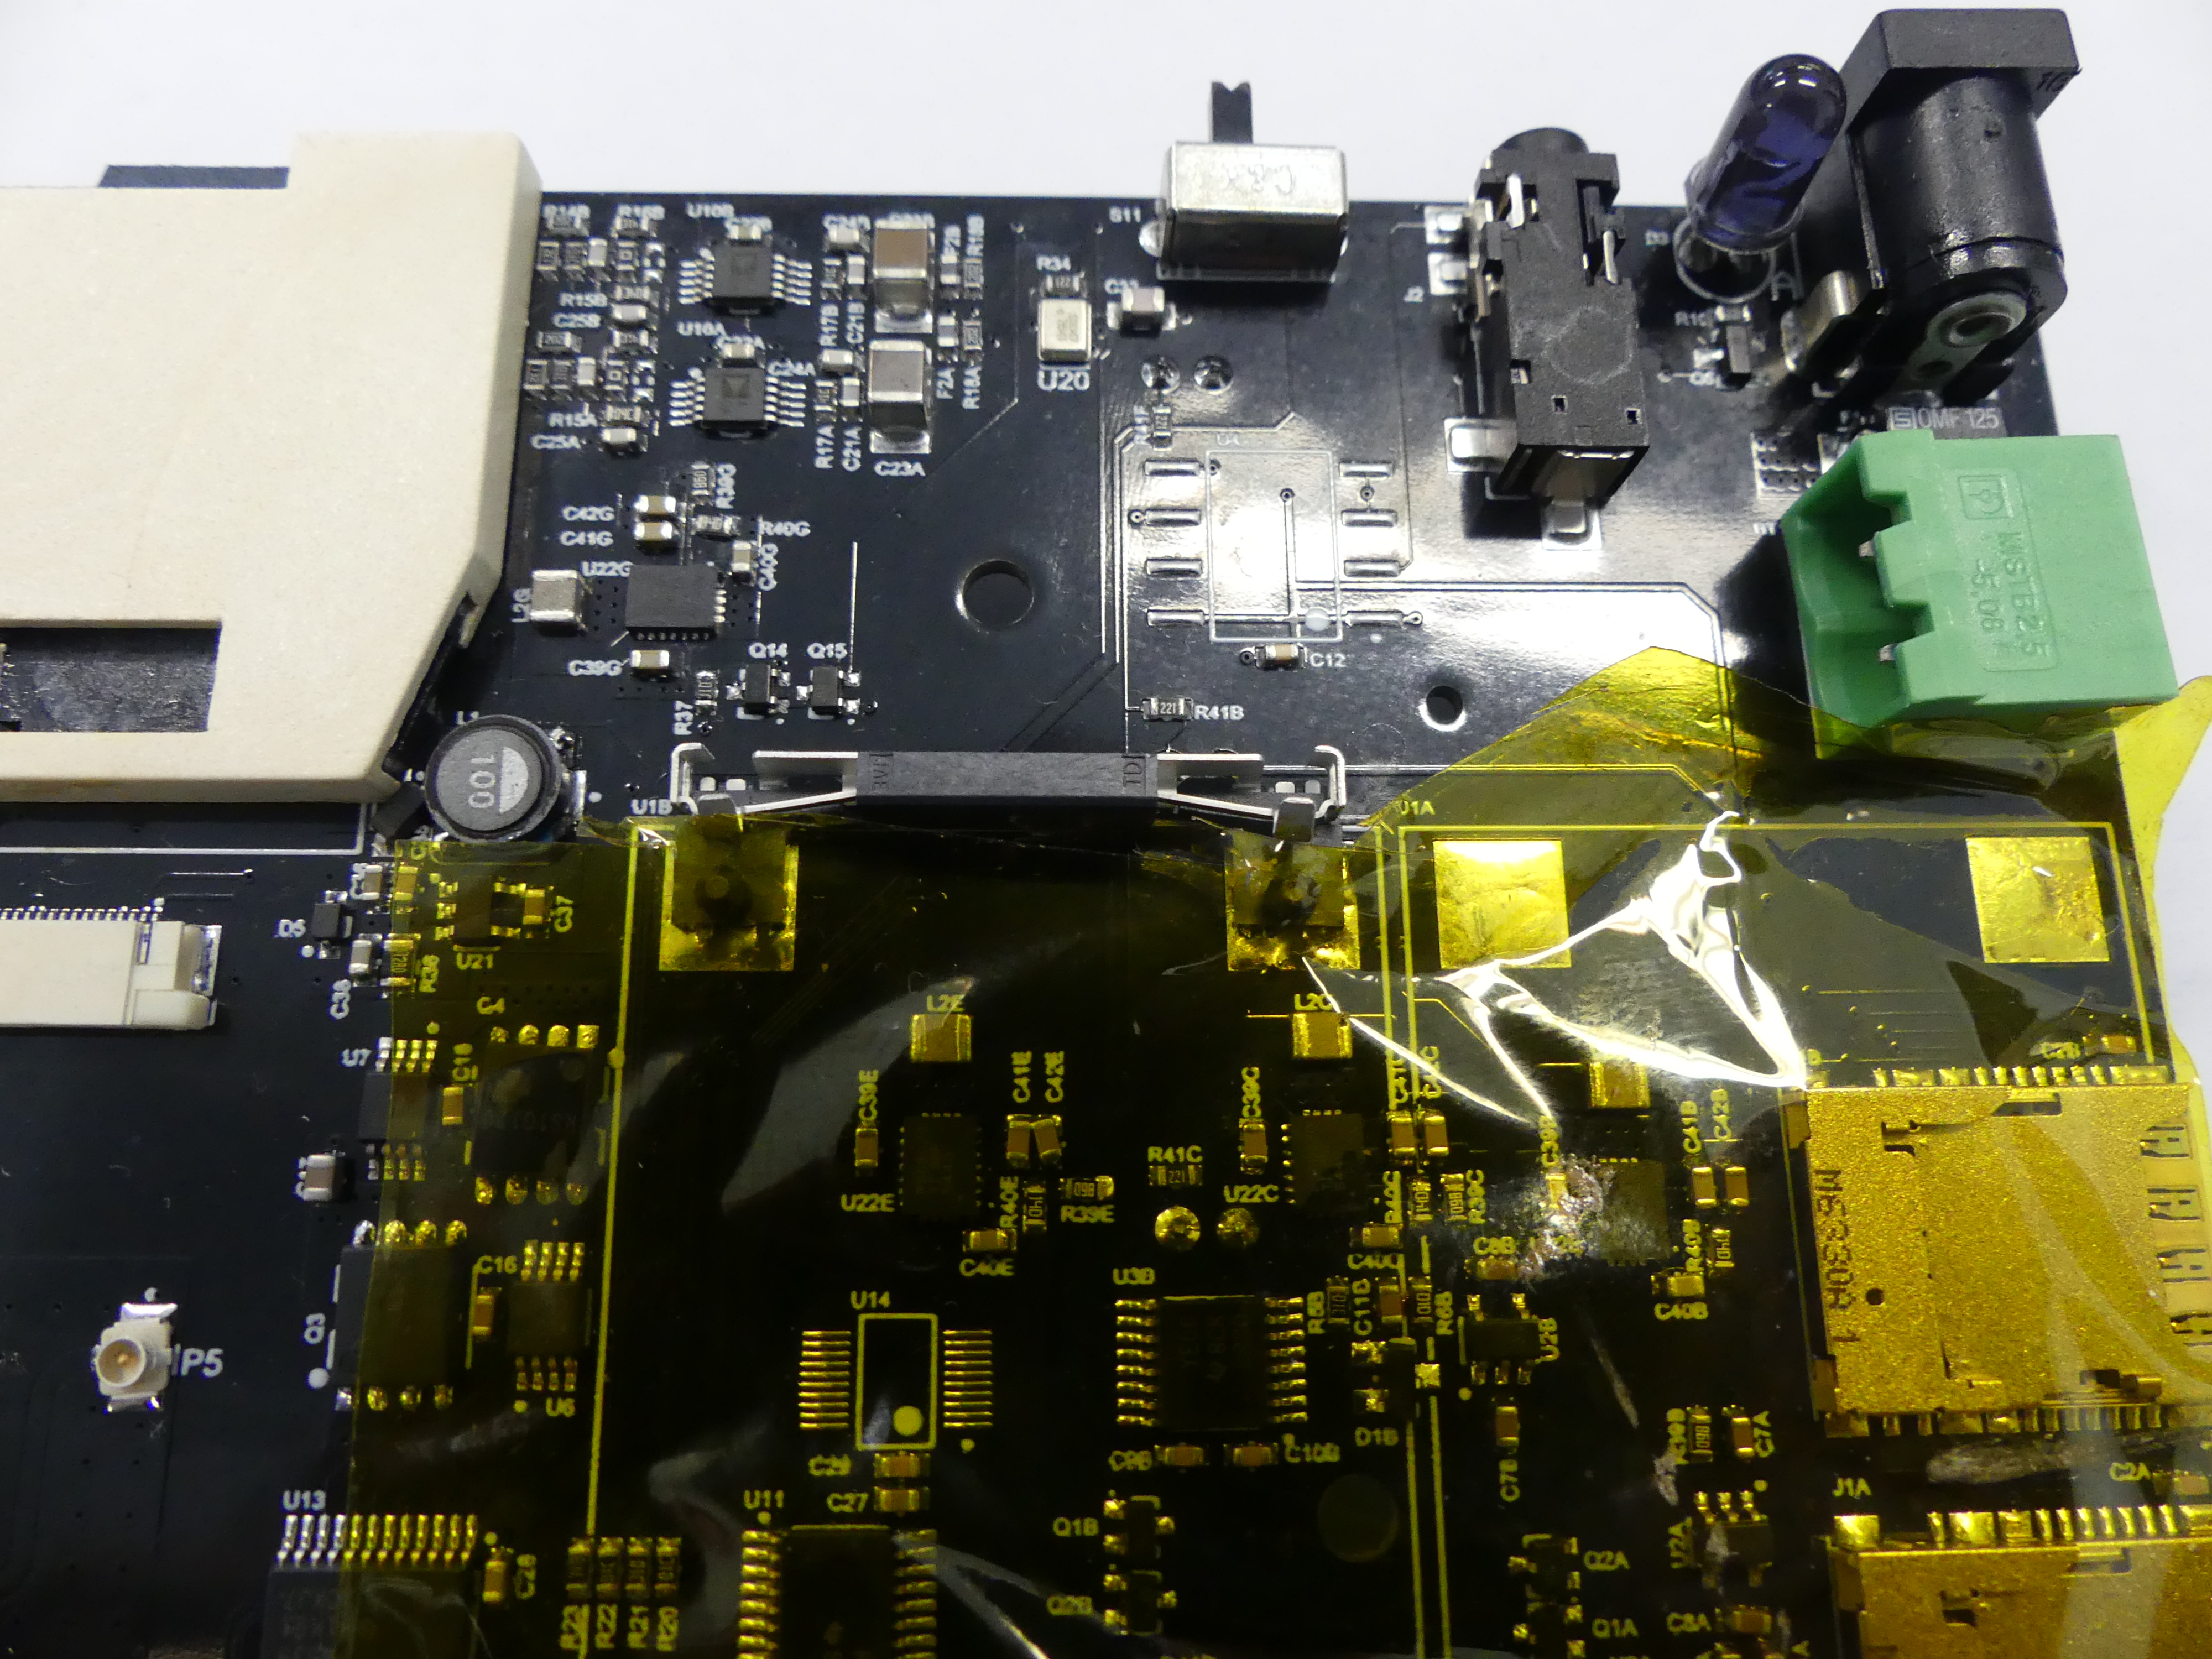
\includegraphics[width=.3\linewidth]{pics/MEGAphone_PCB_r1_U1A} 
\end{center} 
\caption{Close up showing the latch installed in U1B but not U1A.\\}
\label{MEGAphone_PCB_r1_U1A}
\end{figure}

\begin{figure} \begin{center}
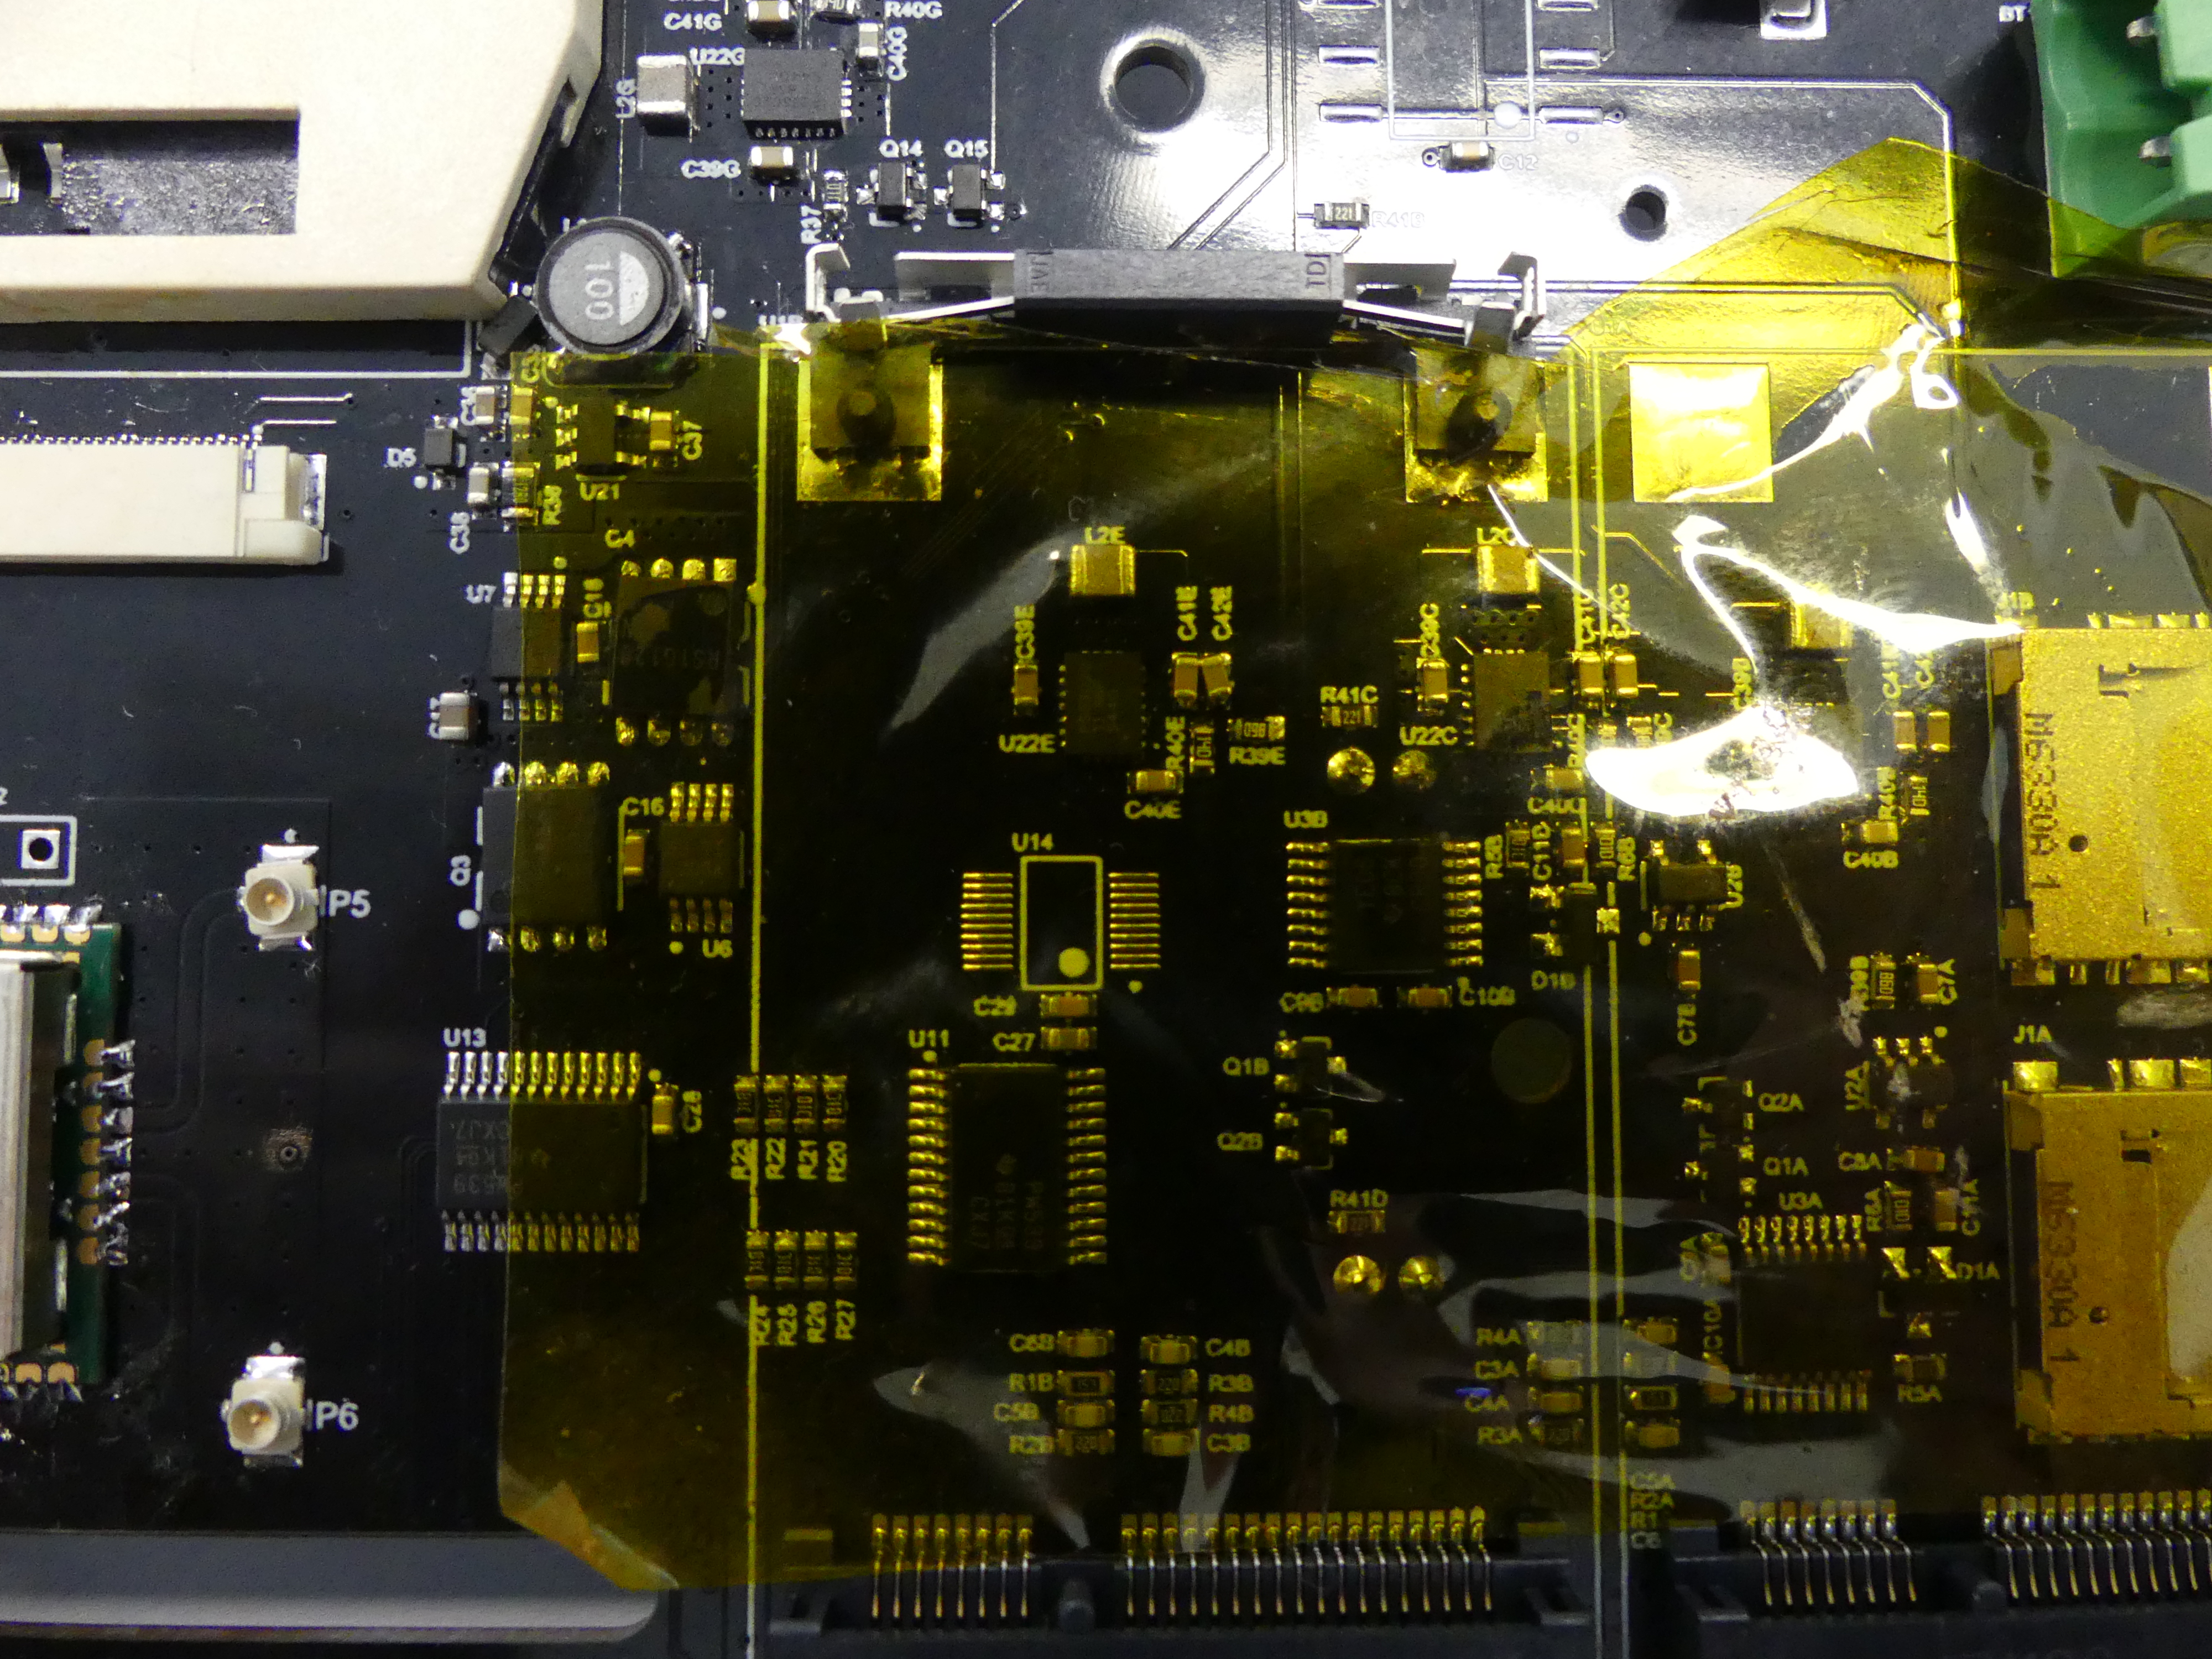
\includegraphics[width=.3\linewidth]{pics/MEGAphone_PCB_r1_U14} 
\end{center} 
\caption{Close up showing unpopulated component U14.\\}
\label{MEGAphone_PCB_r1_U14}
\end{figure}

\begin{figure} \begin{center}
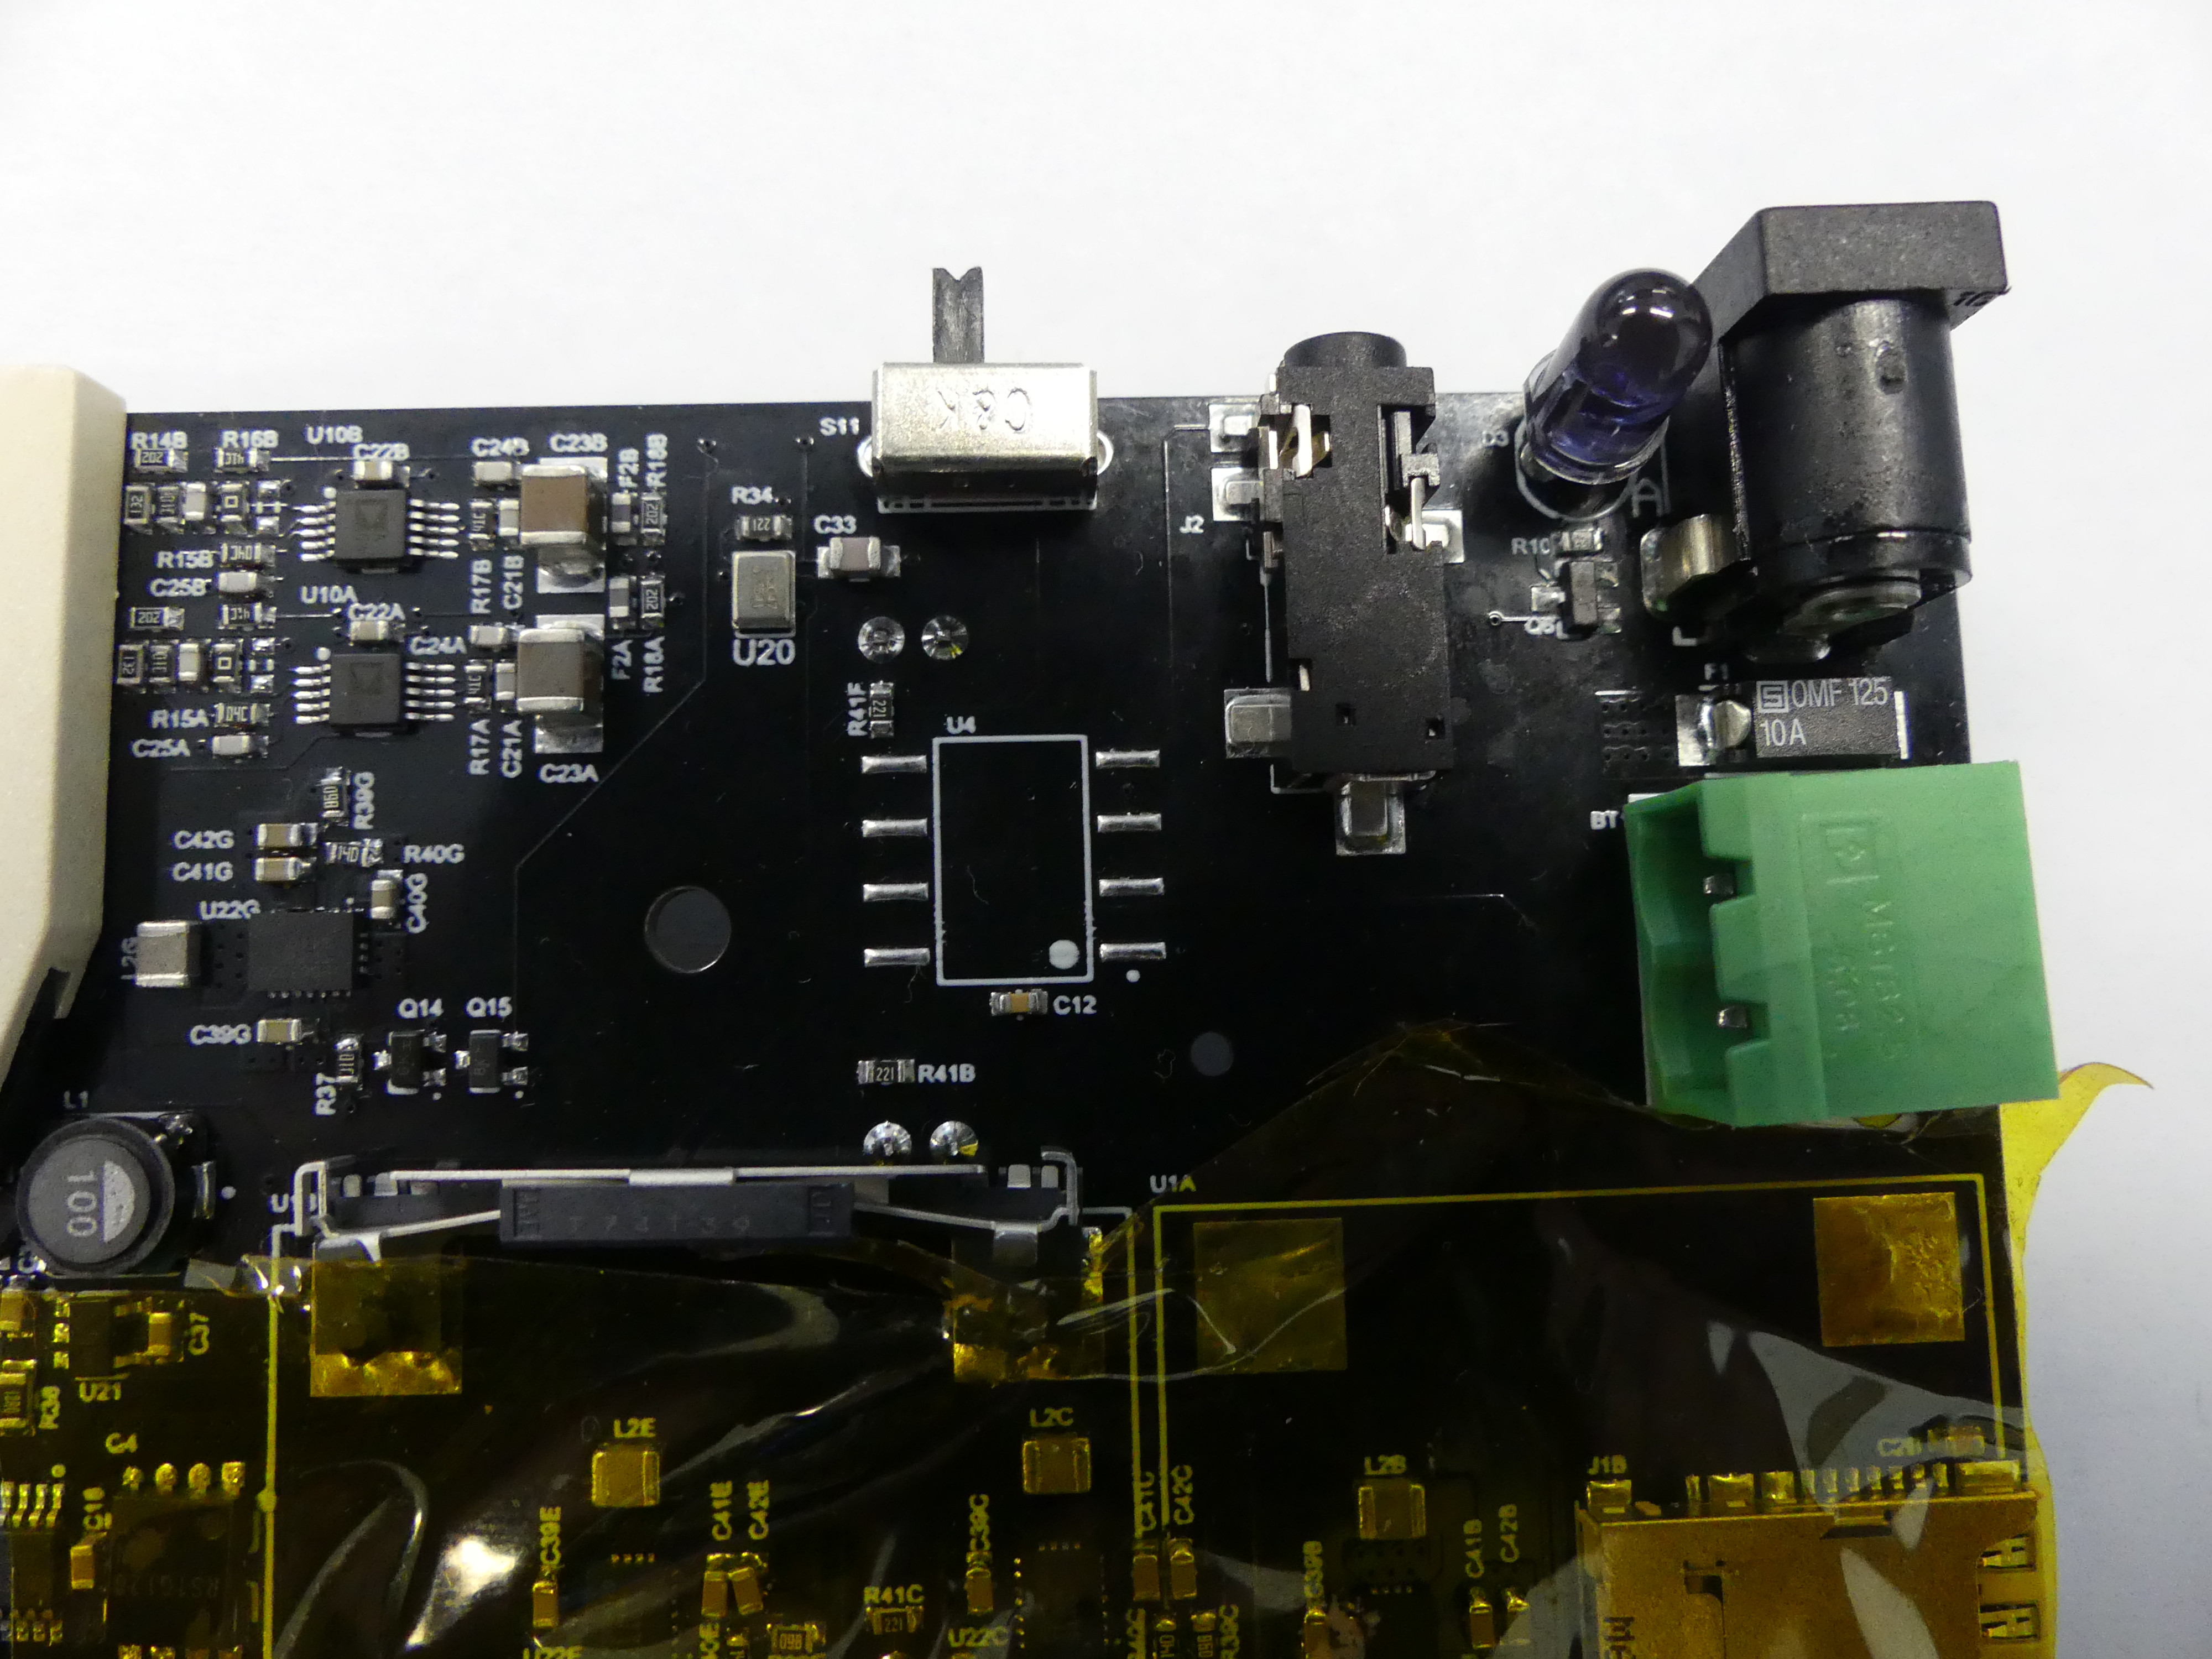
\includegraphics[width=.3\linewidth]{pics/MEGAphone_PCB_r1_U4} 
\end{center} 
\caption{Close up showing unpopulated component U4.\\}
\label{MEGAphone_PCB_r1_U4}
\end{figure}

\begin{figure} \begin{center}
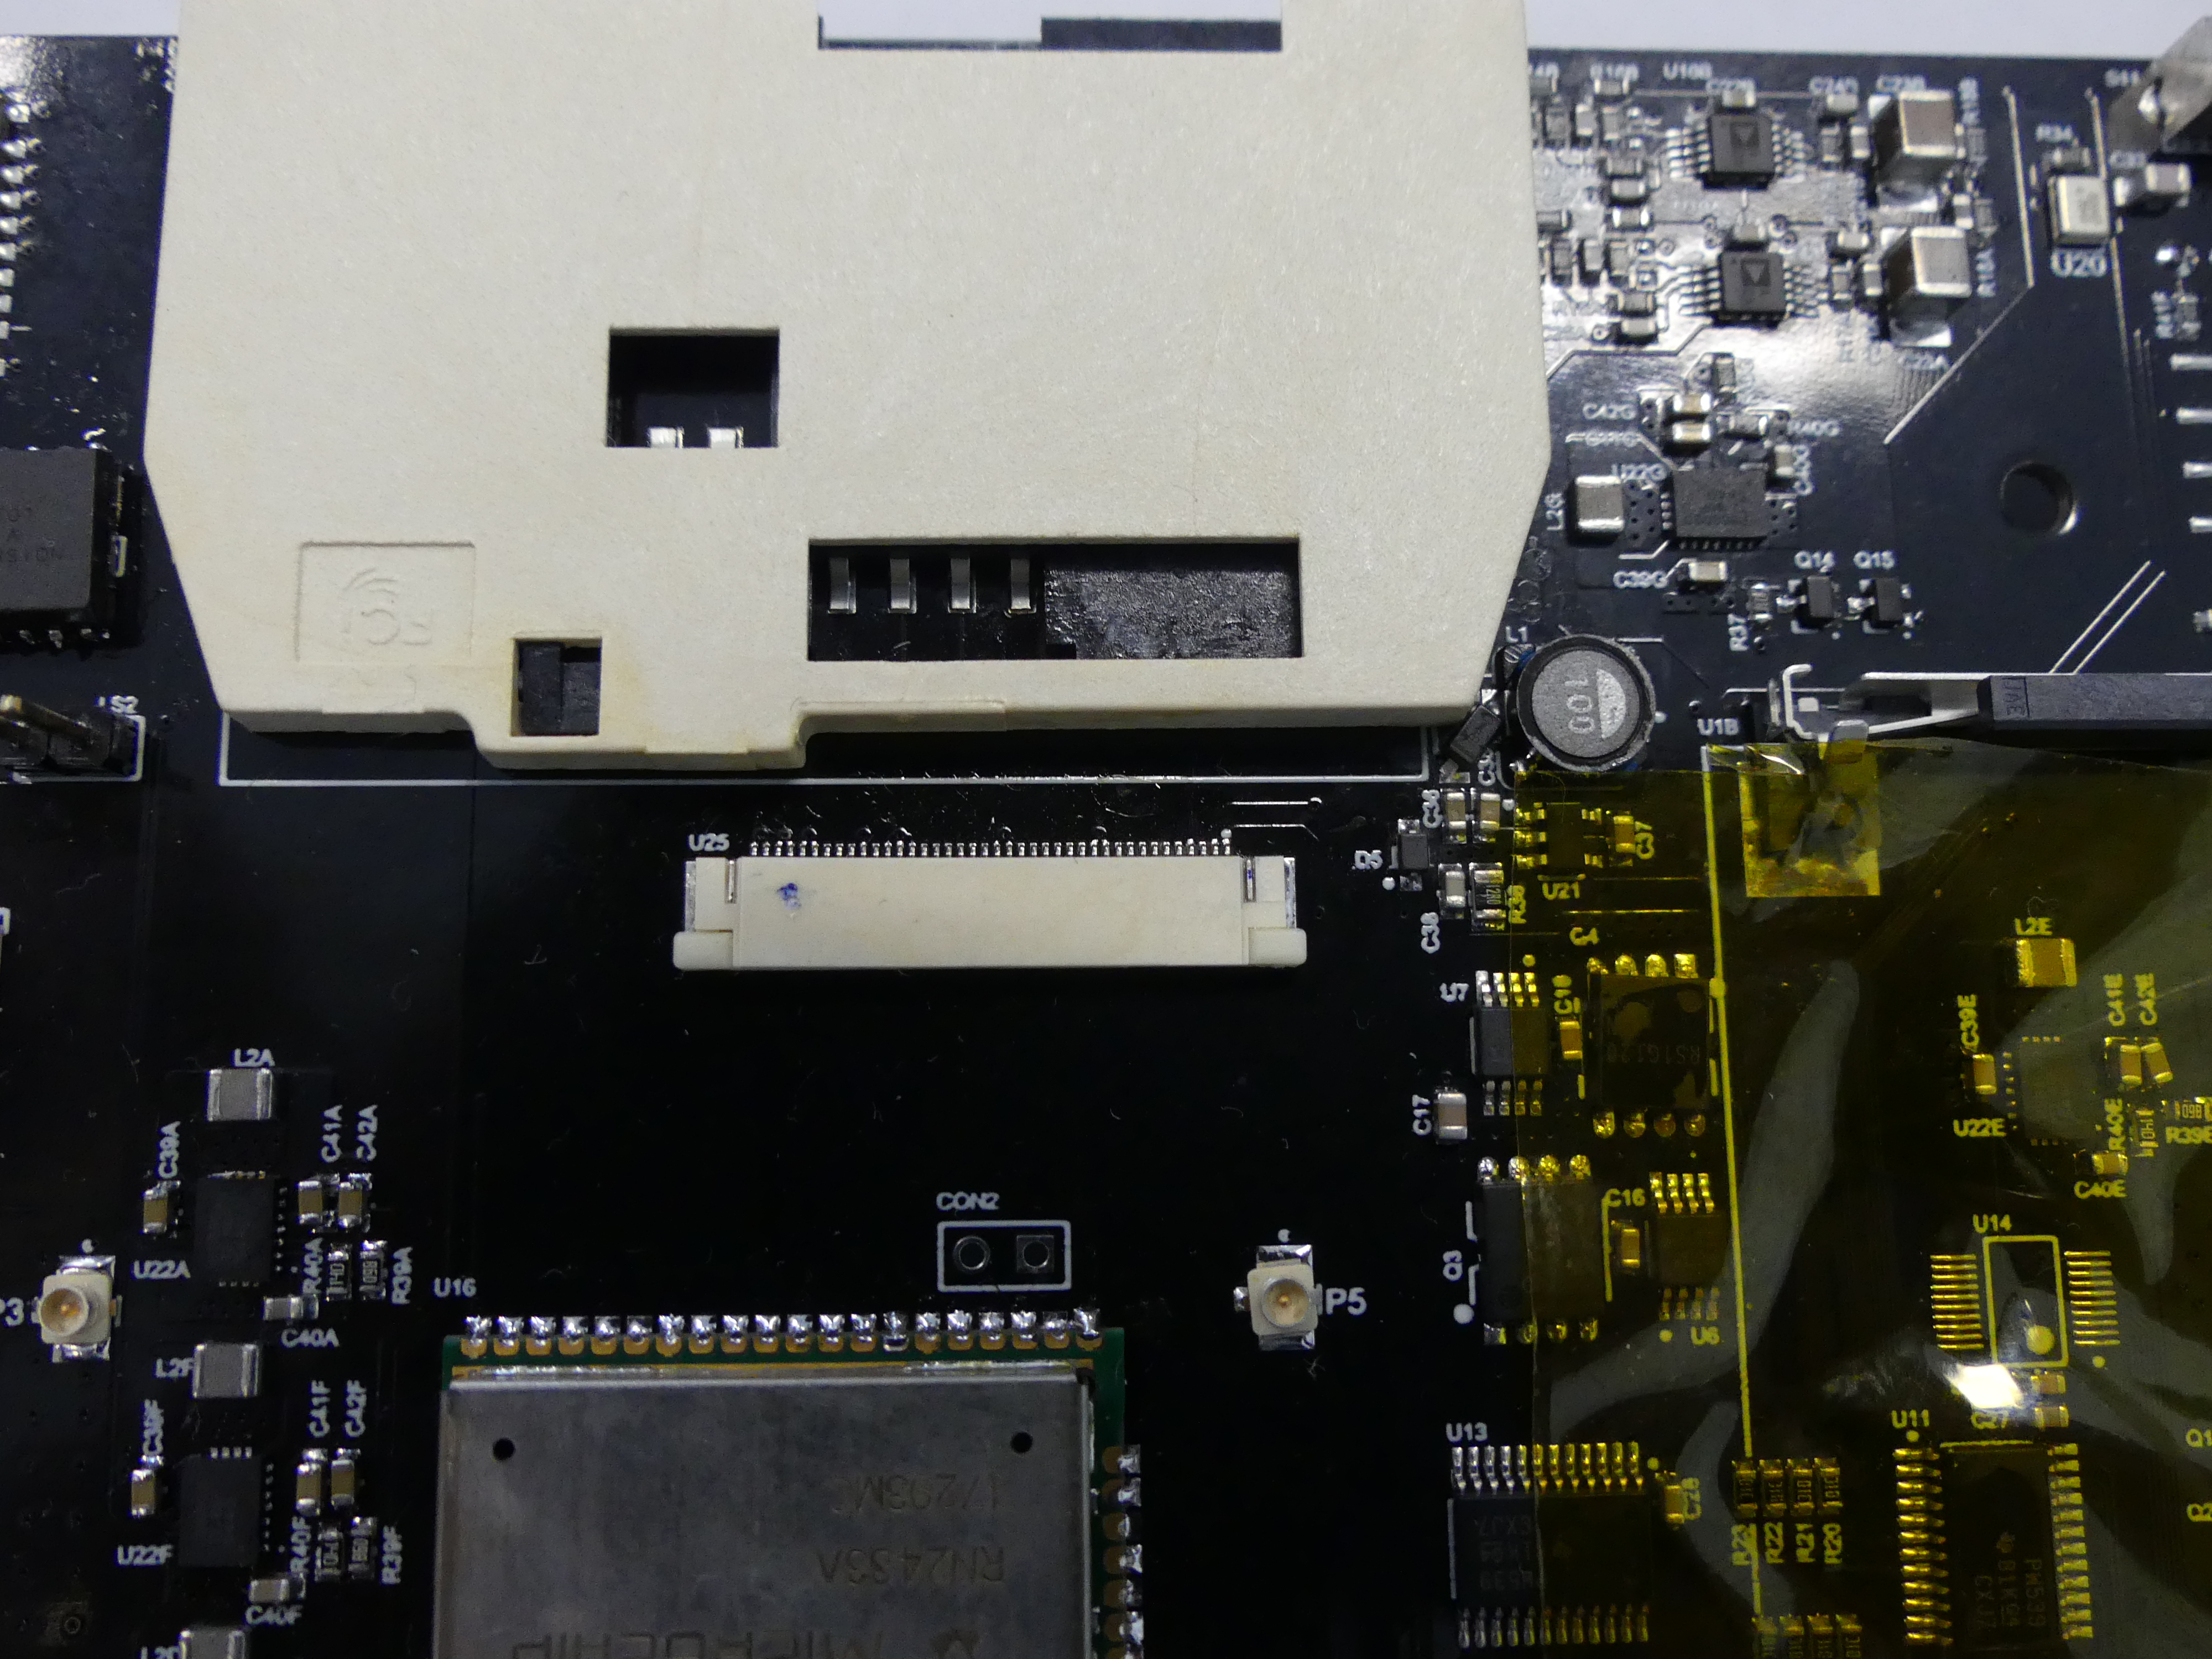
\includegraphics[width=.3\linewidth]{pics/MEGAphone_PCB_r1_U25}
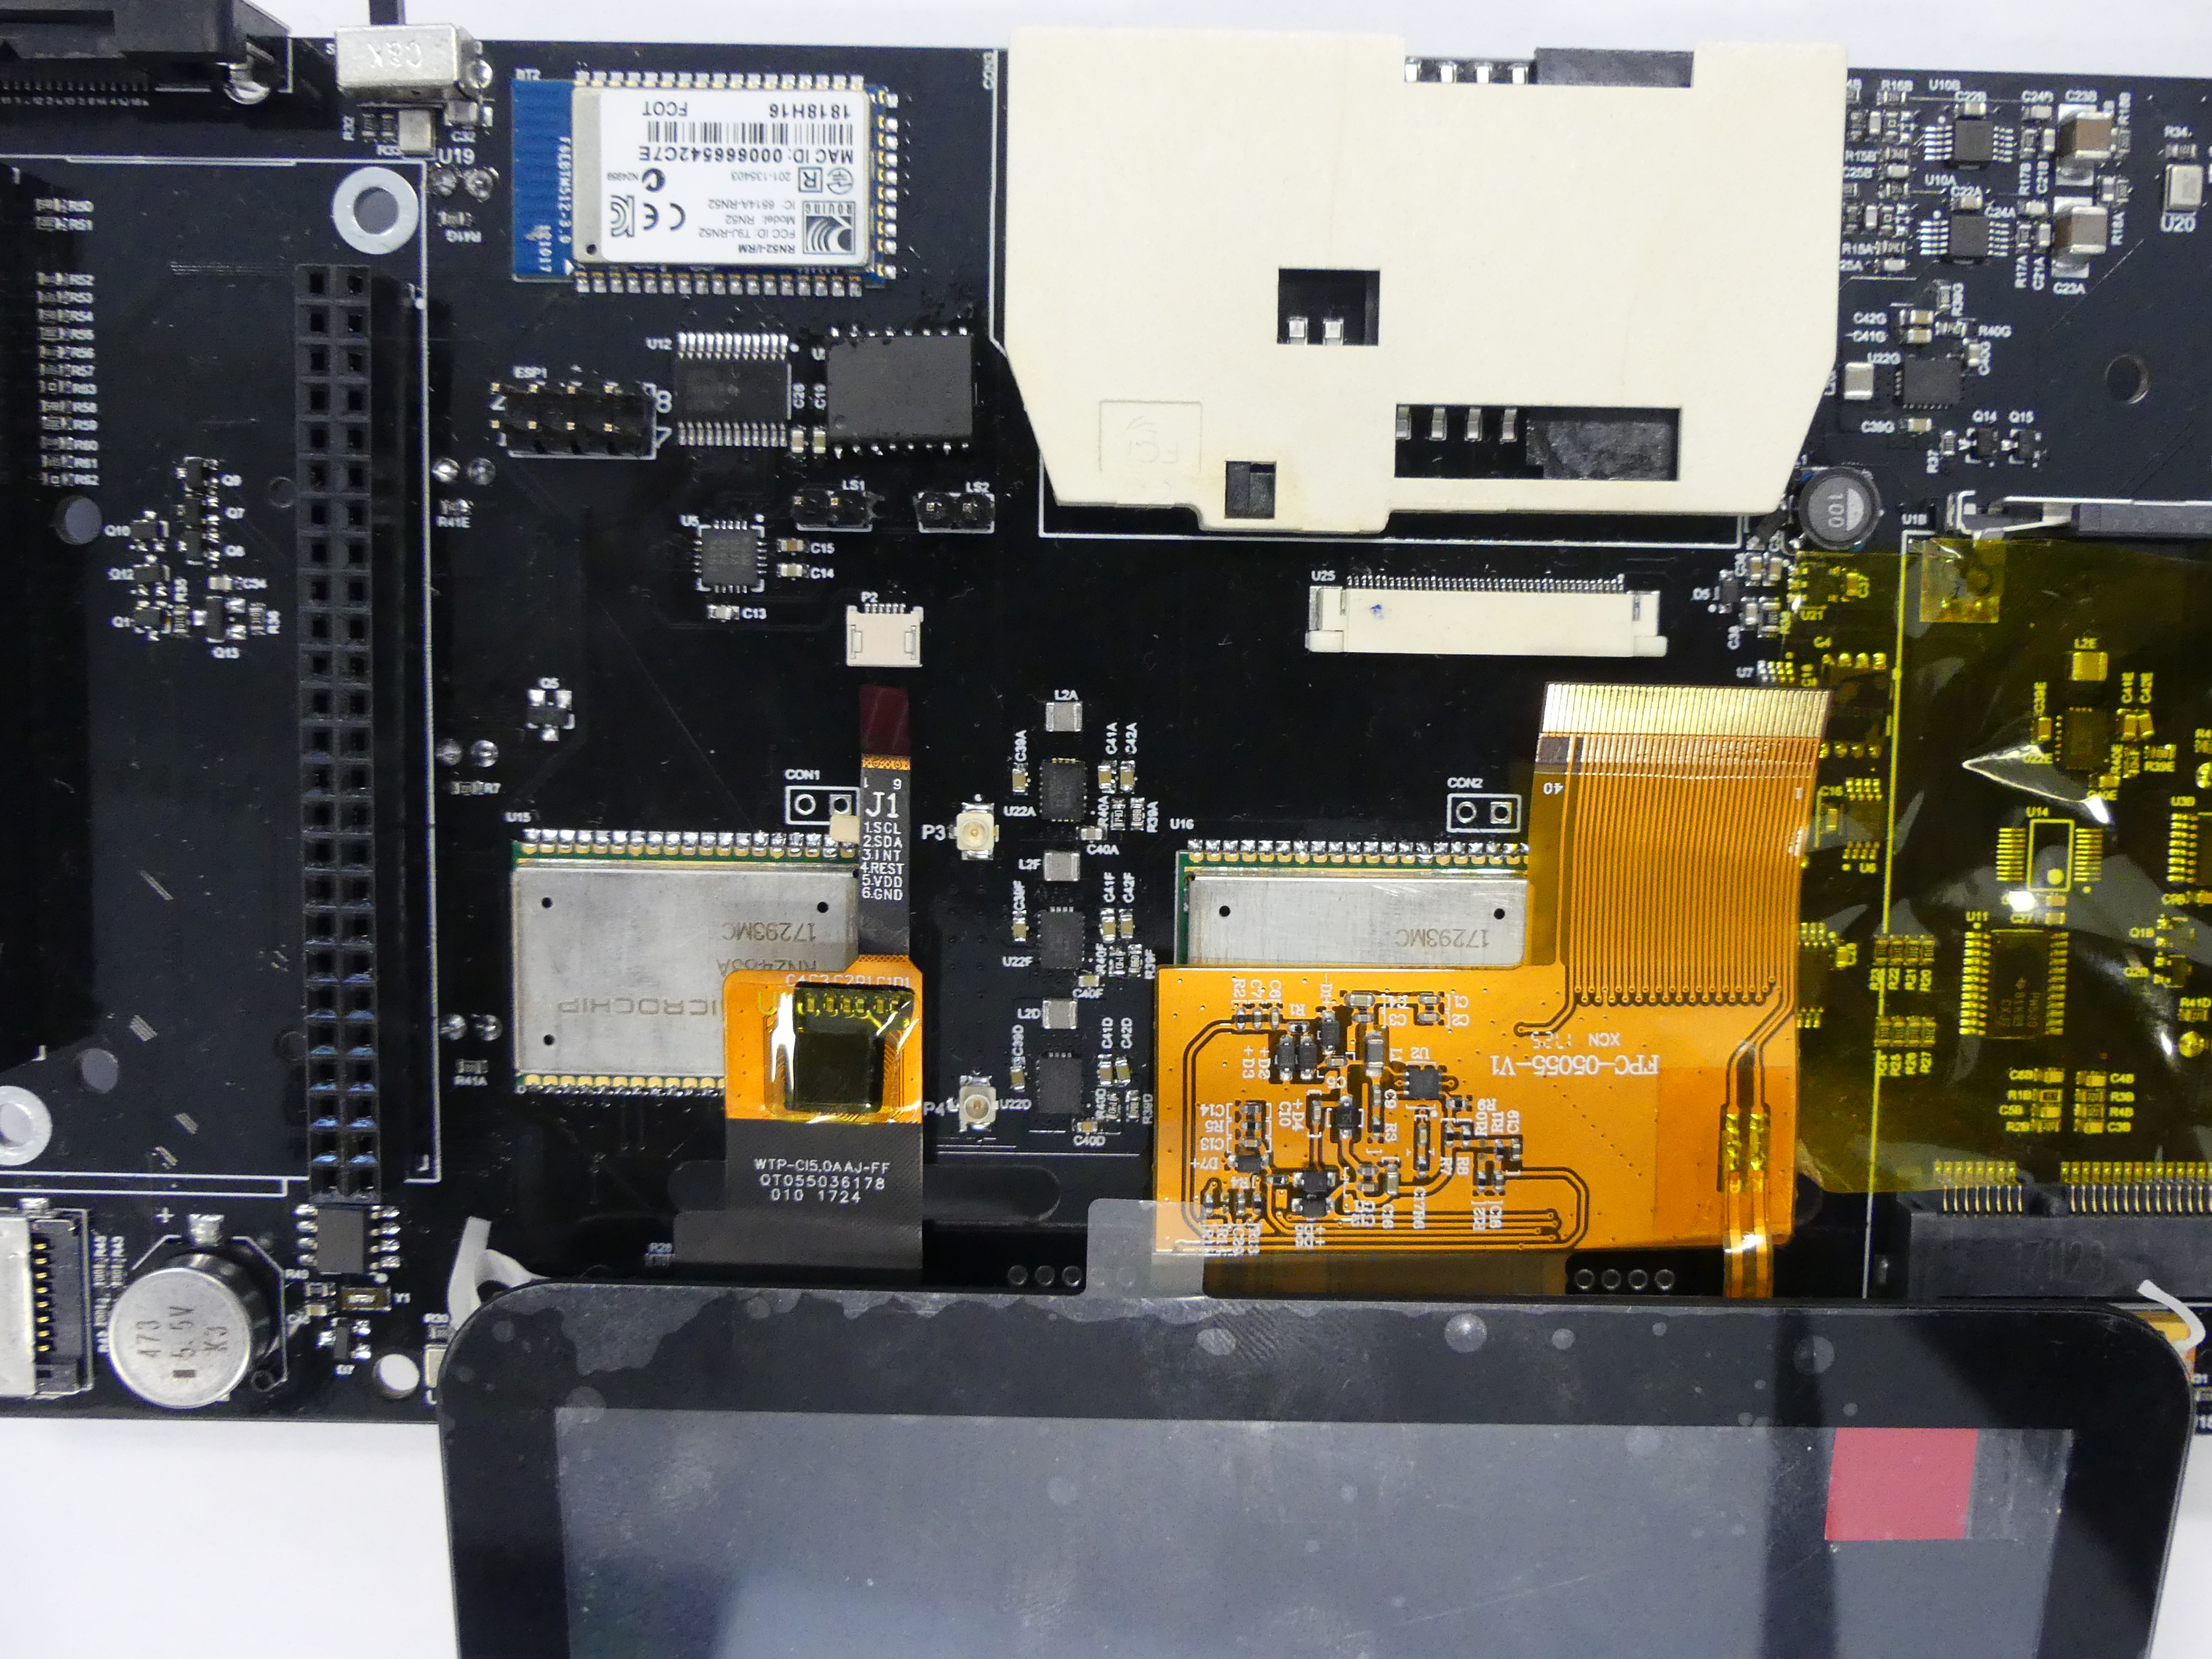
\includegraphics[width=.3\linewidth]{pics/MEGAphone_PCB_r1_U25_P2_ribbon}
\end{center} 
\caption{Close up showing component U25 as well with as the ribbon connector for the screen. U25 needs to be re-positioned.\\}
\label{MEGAphone_PCB_r1_U25}
\end{figure}

\begin{figure} \begin{center}
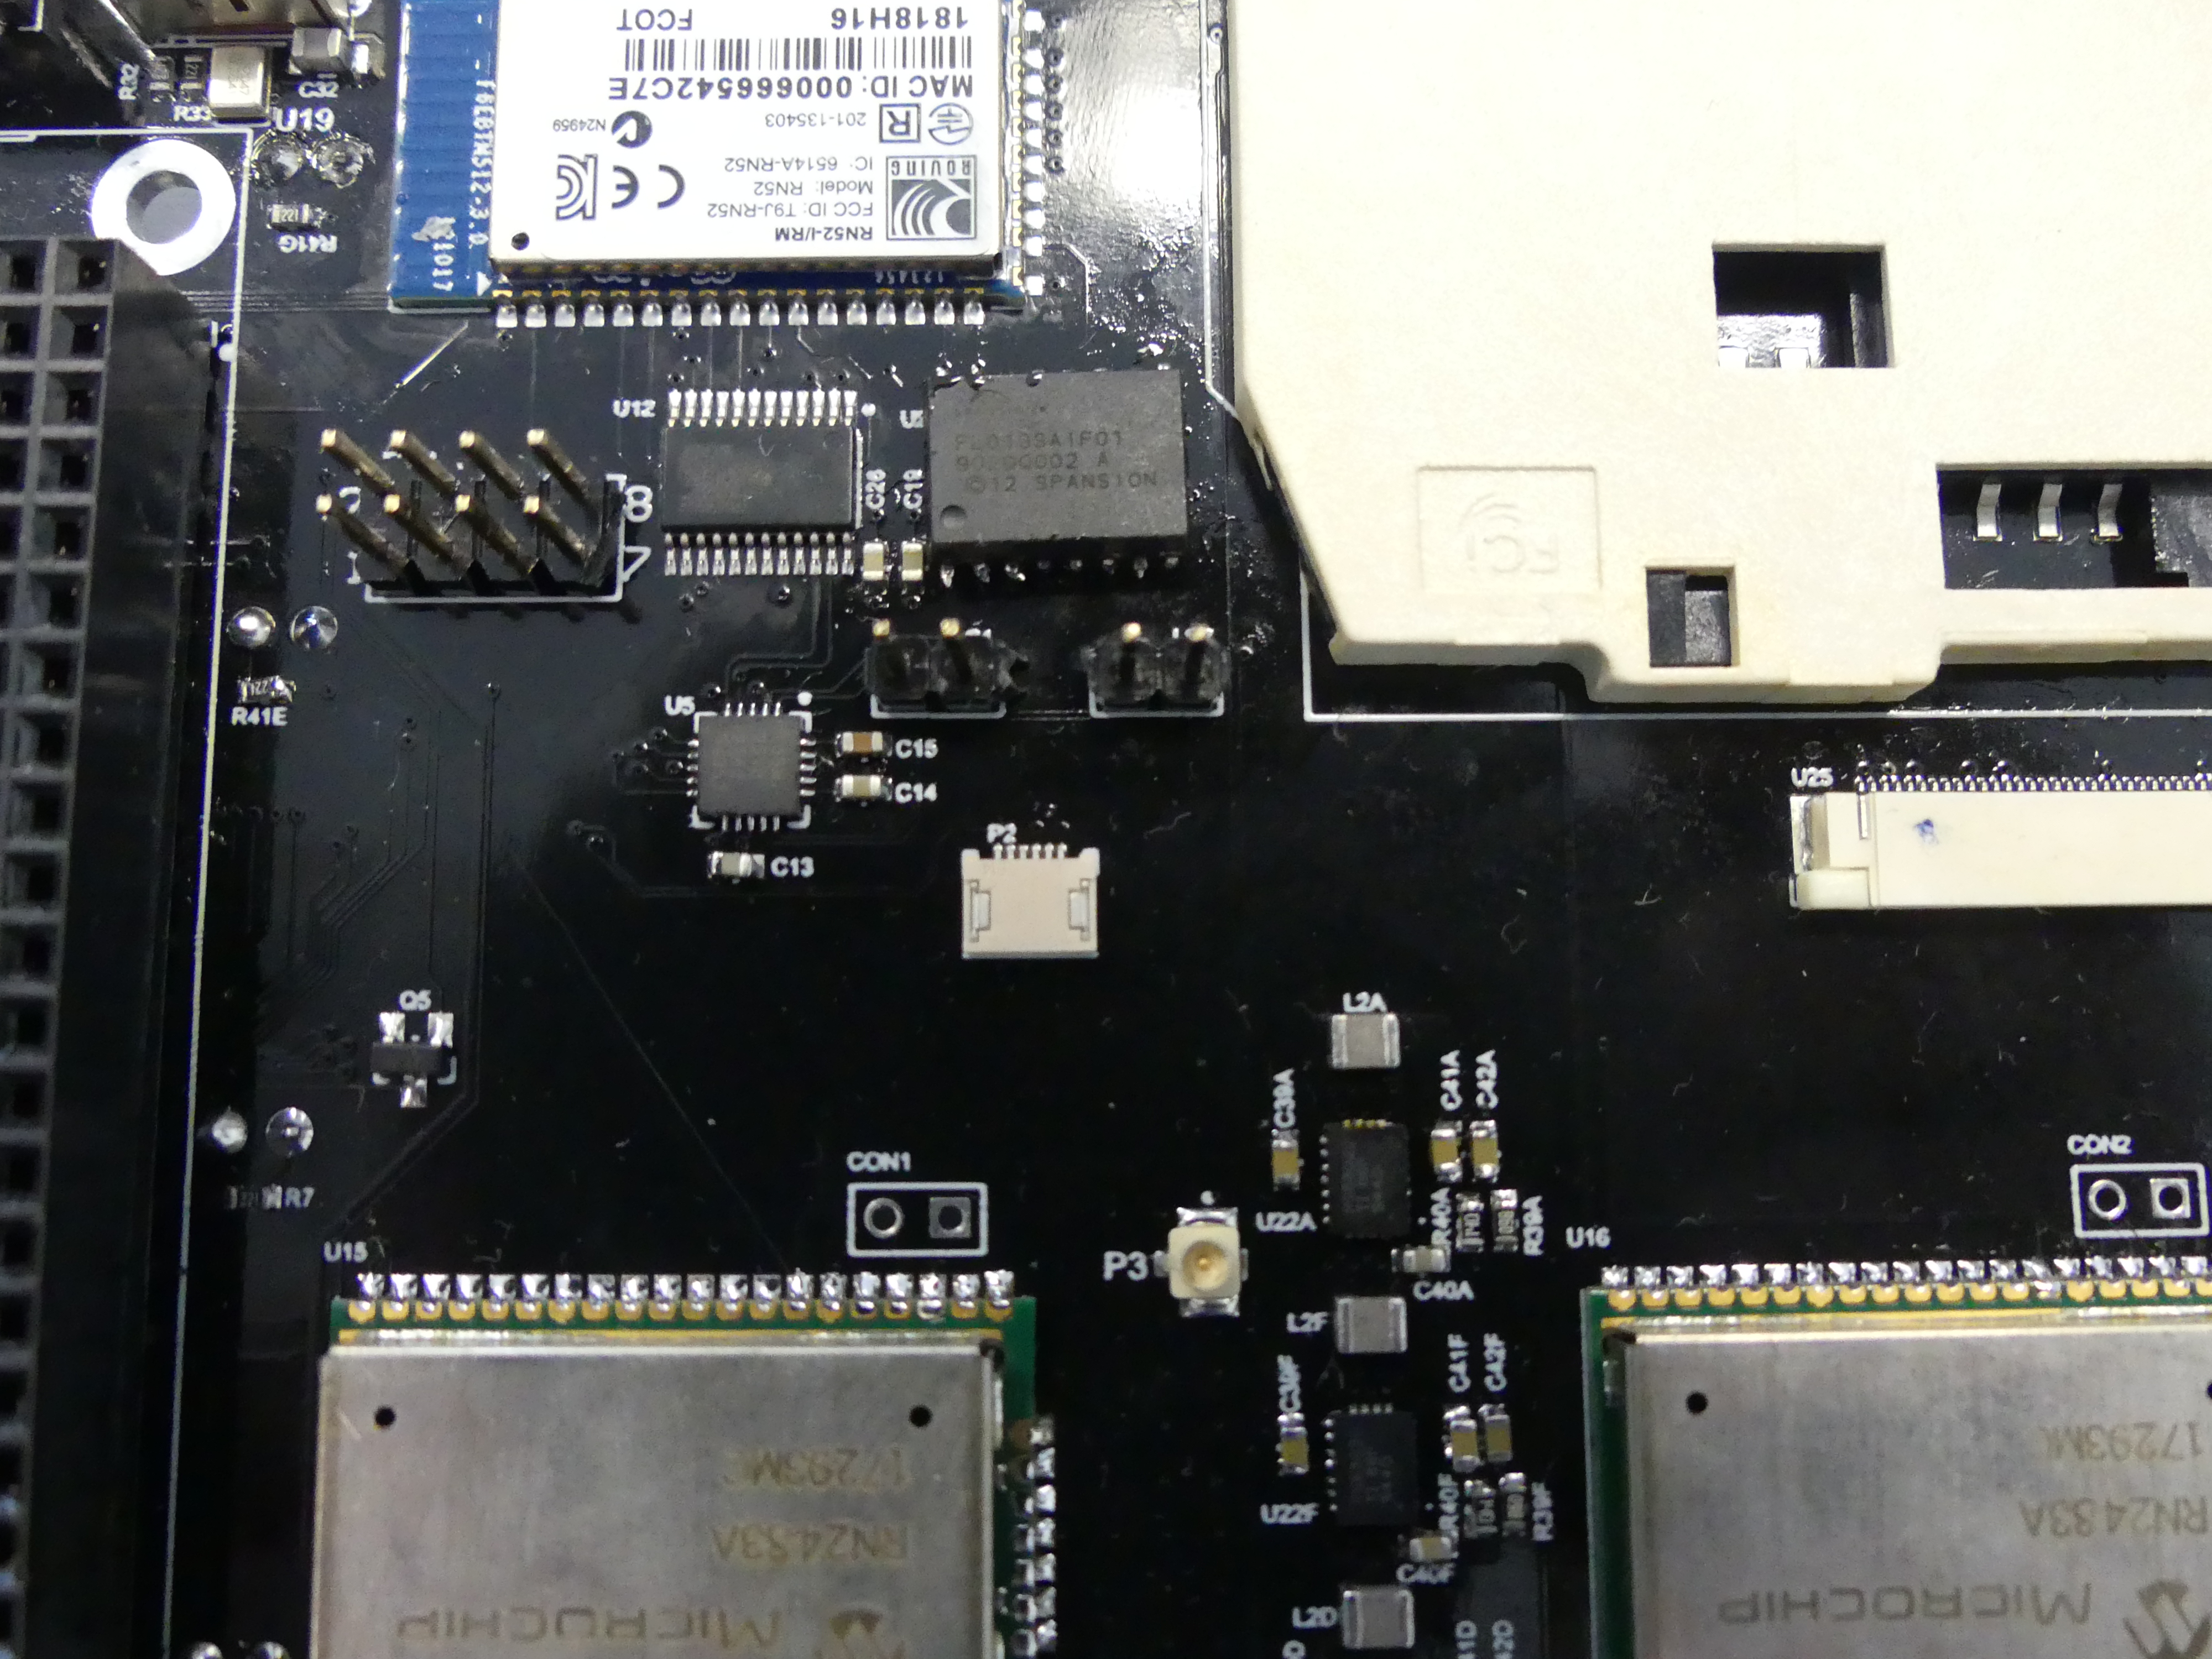
\includegraphics[width=.3\linewidth]{pics/MEGAphone_PCB_r1_P2}
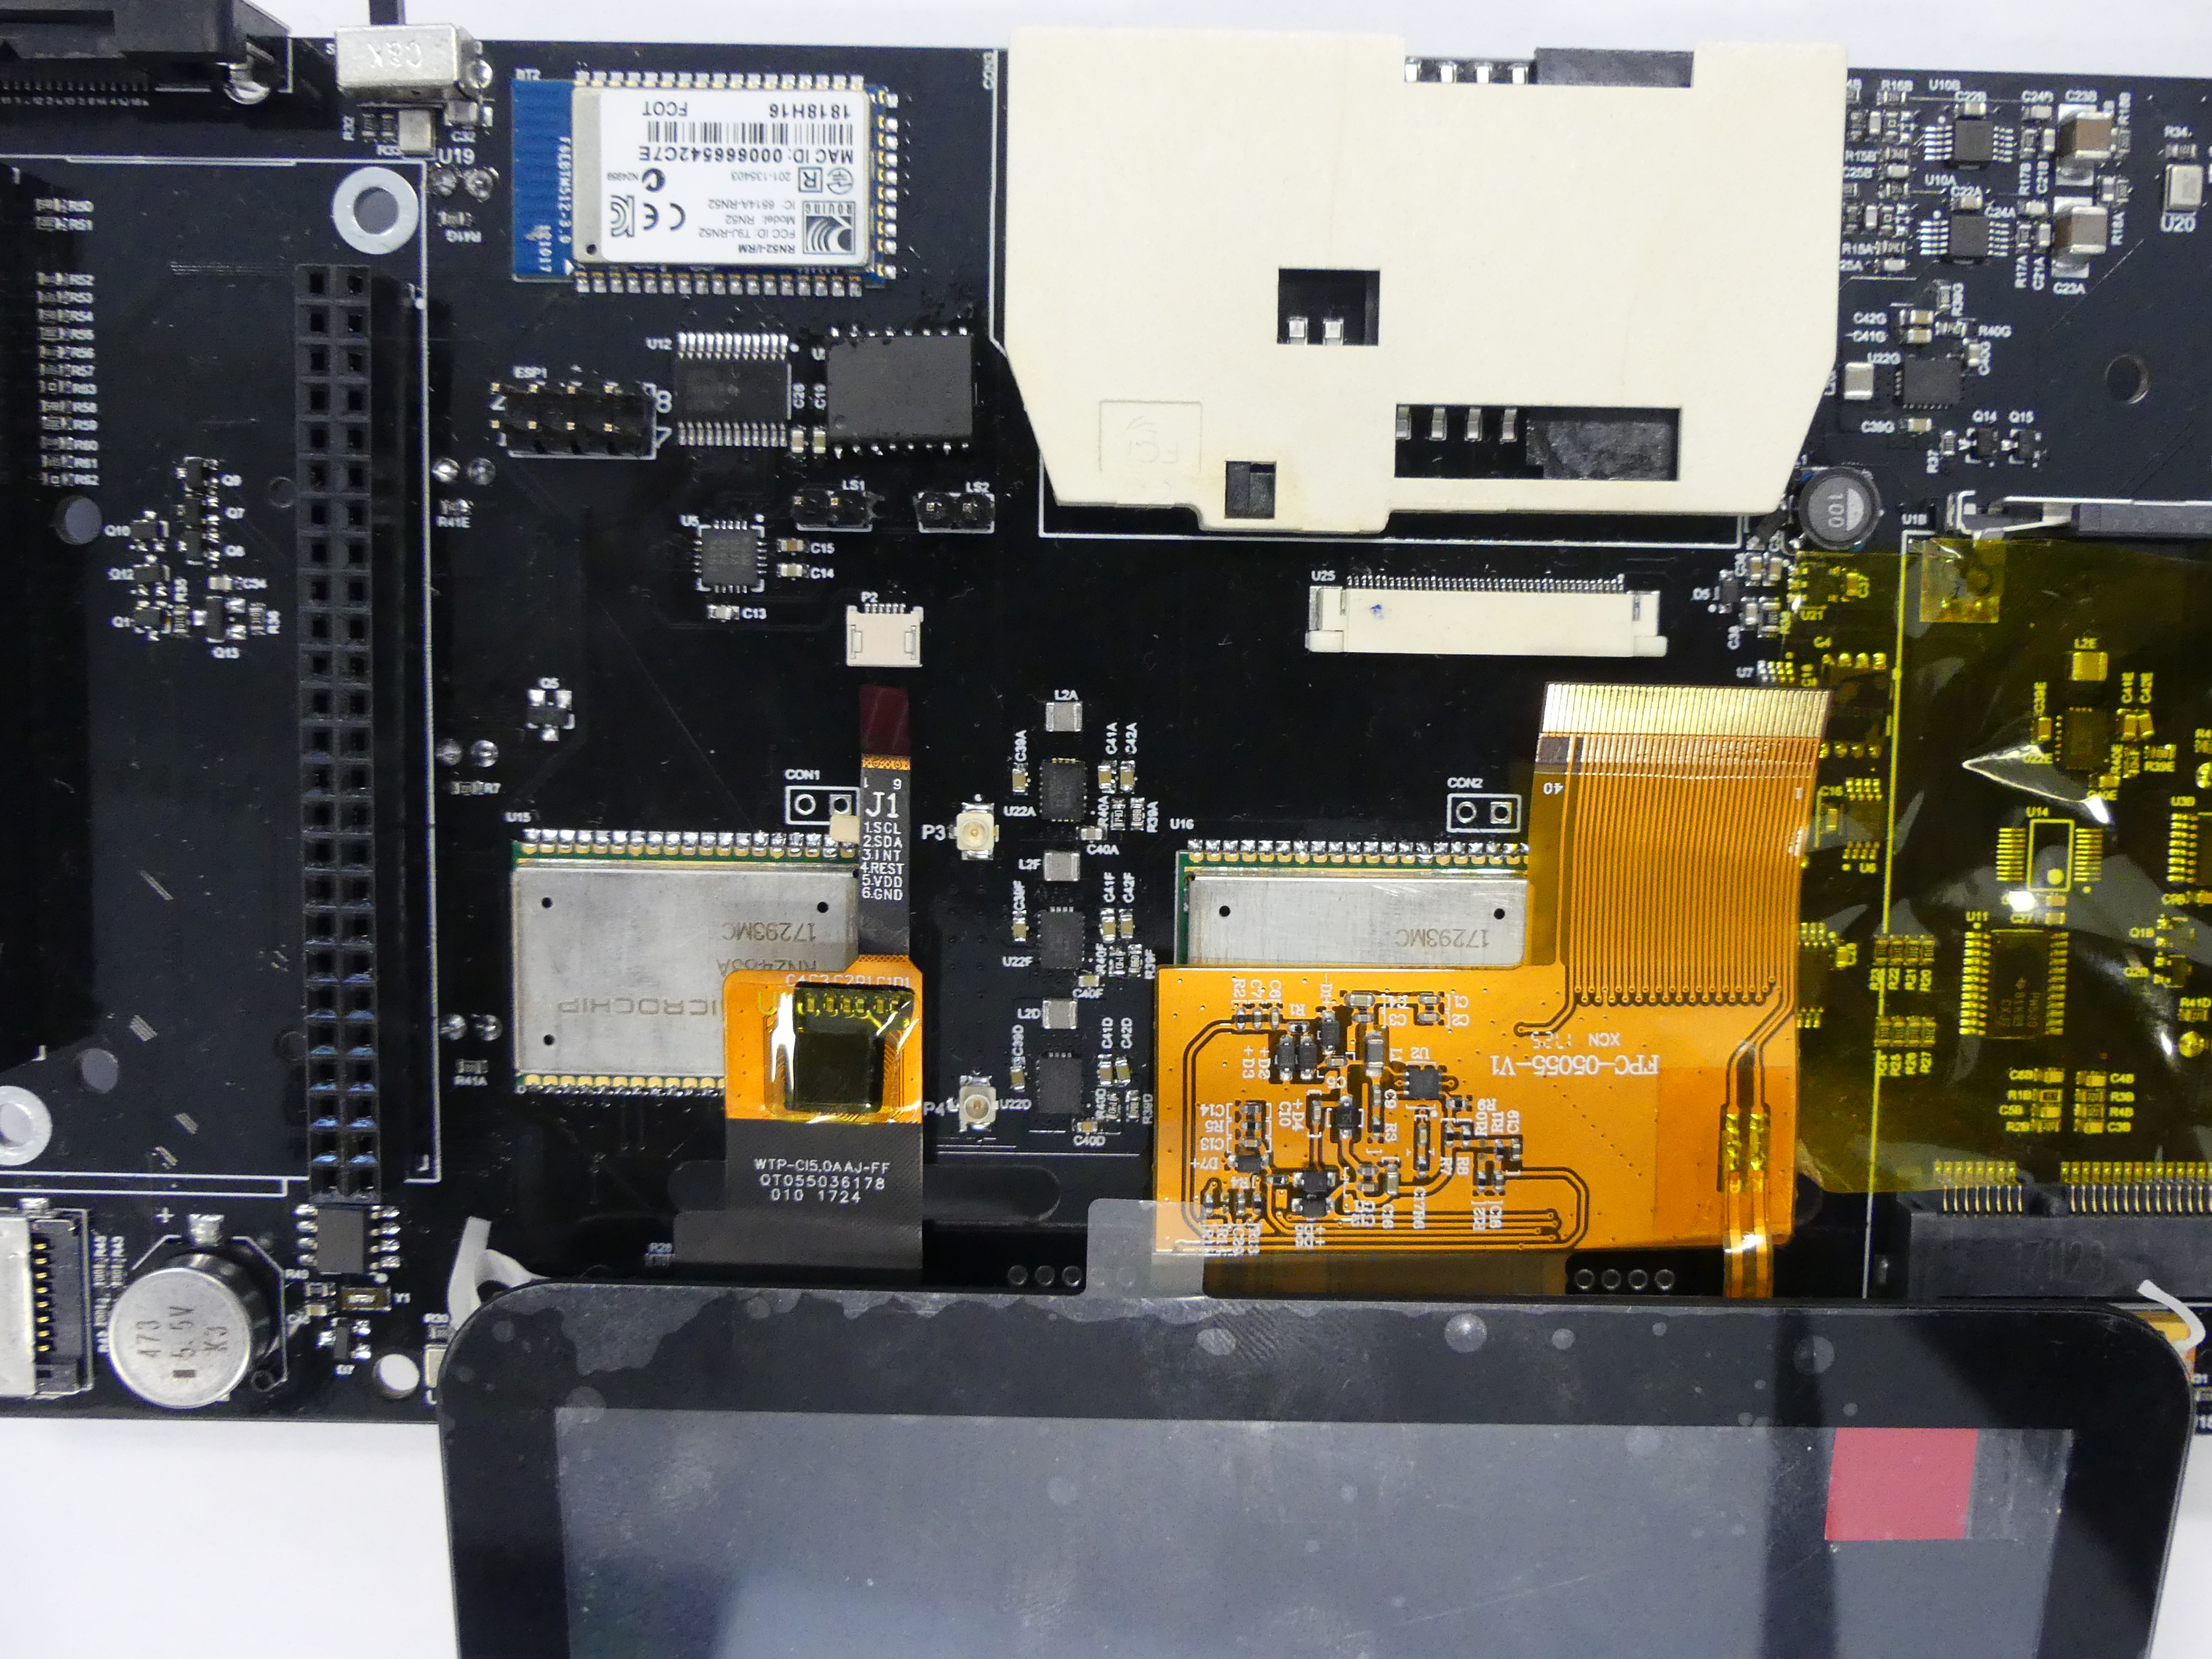
\includegraphics[width=.3\linewidth]{pics/MEGAphone_PCB_r1_U25_P2_ribbon}
\end{center} 
\caption{Close up showing component P2 as well with as the ribbon connector for the screen. P2 needs to be re-positioned. \\}
\label{MEGAphone_PCB_r1_P2}
\end{figure}

\begin{figure} \begin{center}
\includegraphics[width=.3\linewidth]{pics/MEGAphone_PCB_r1_LED1}
\includegraphics[width=.3\linewidth]{pics/MEGAphone_PCB_r1_LED2}
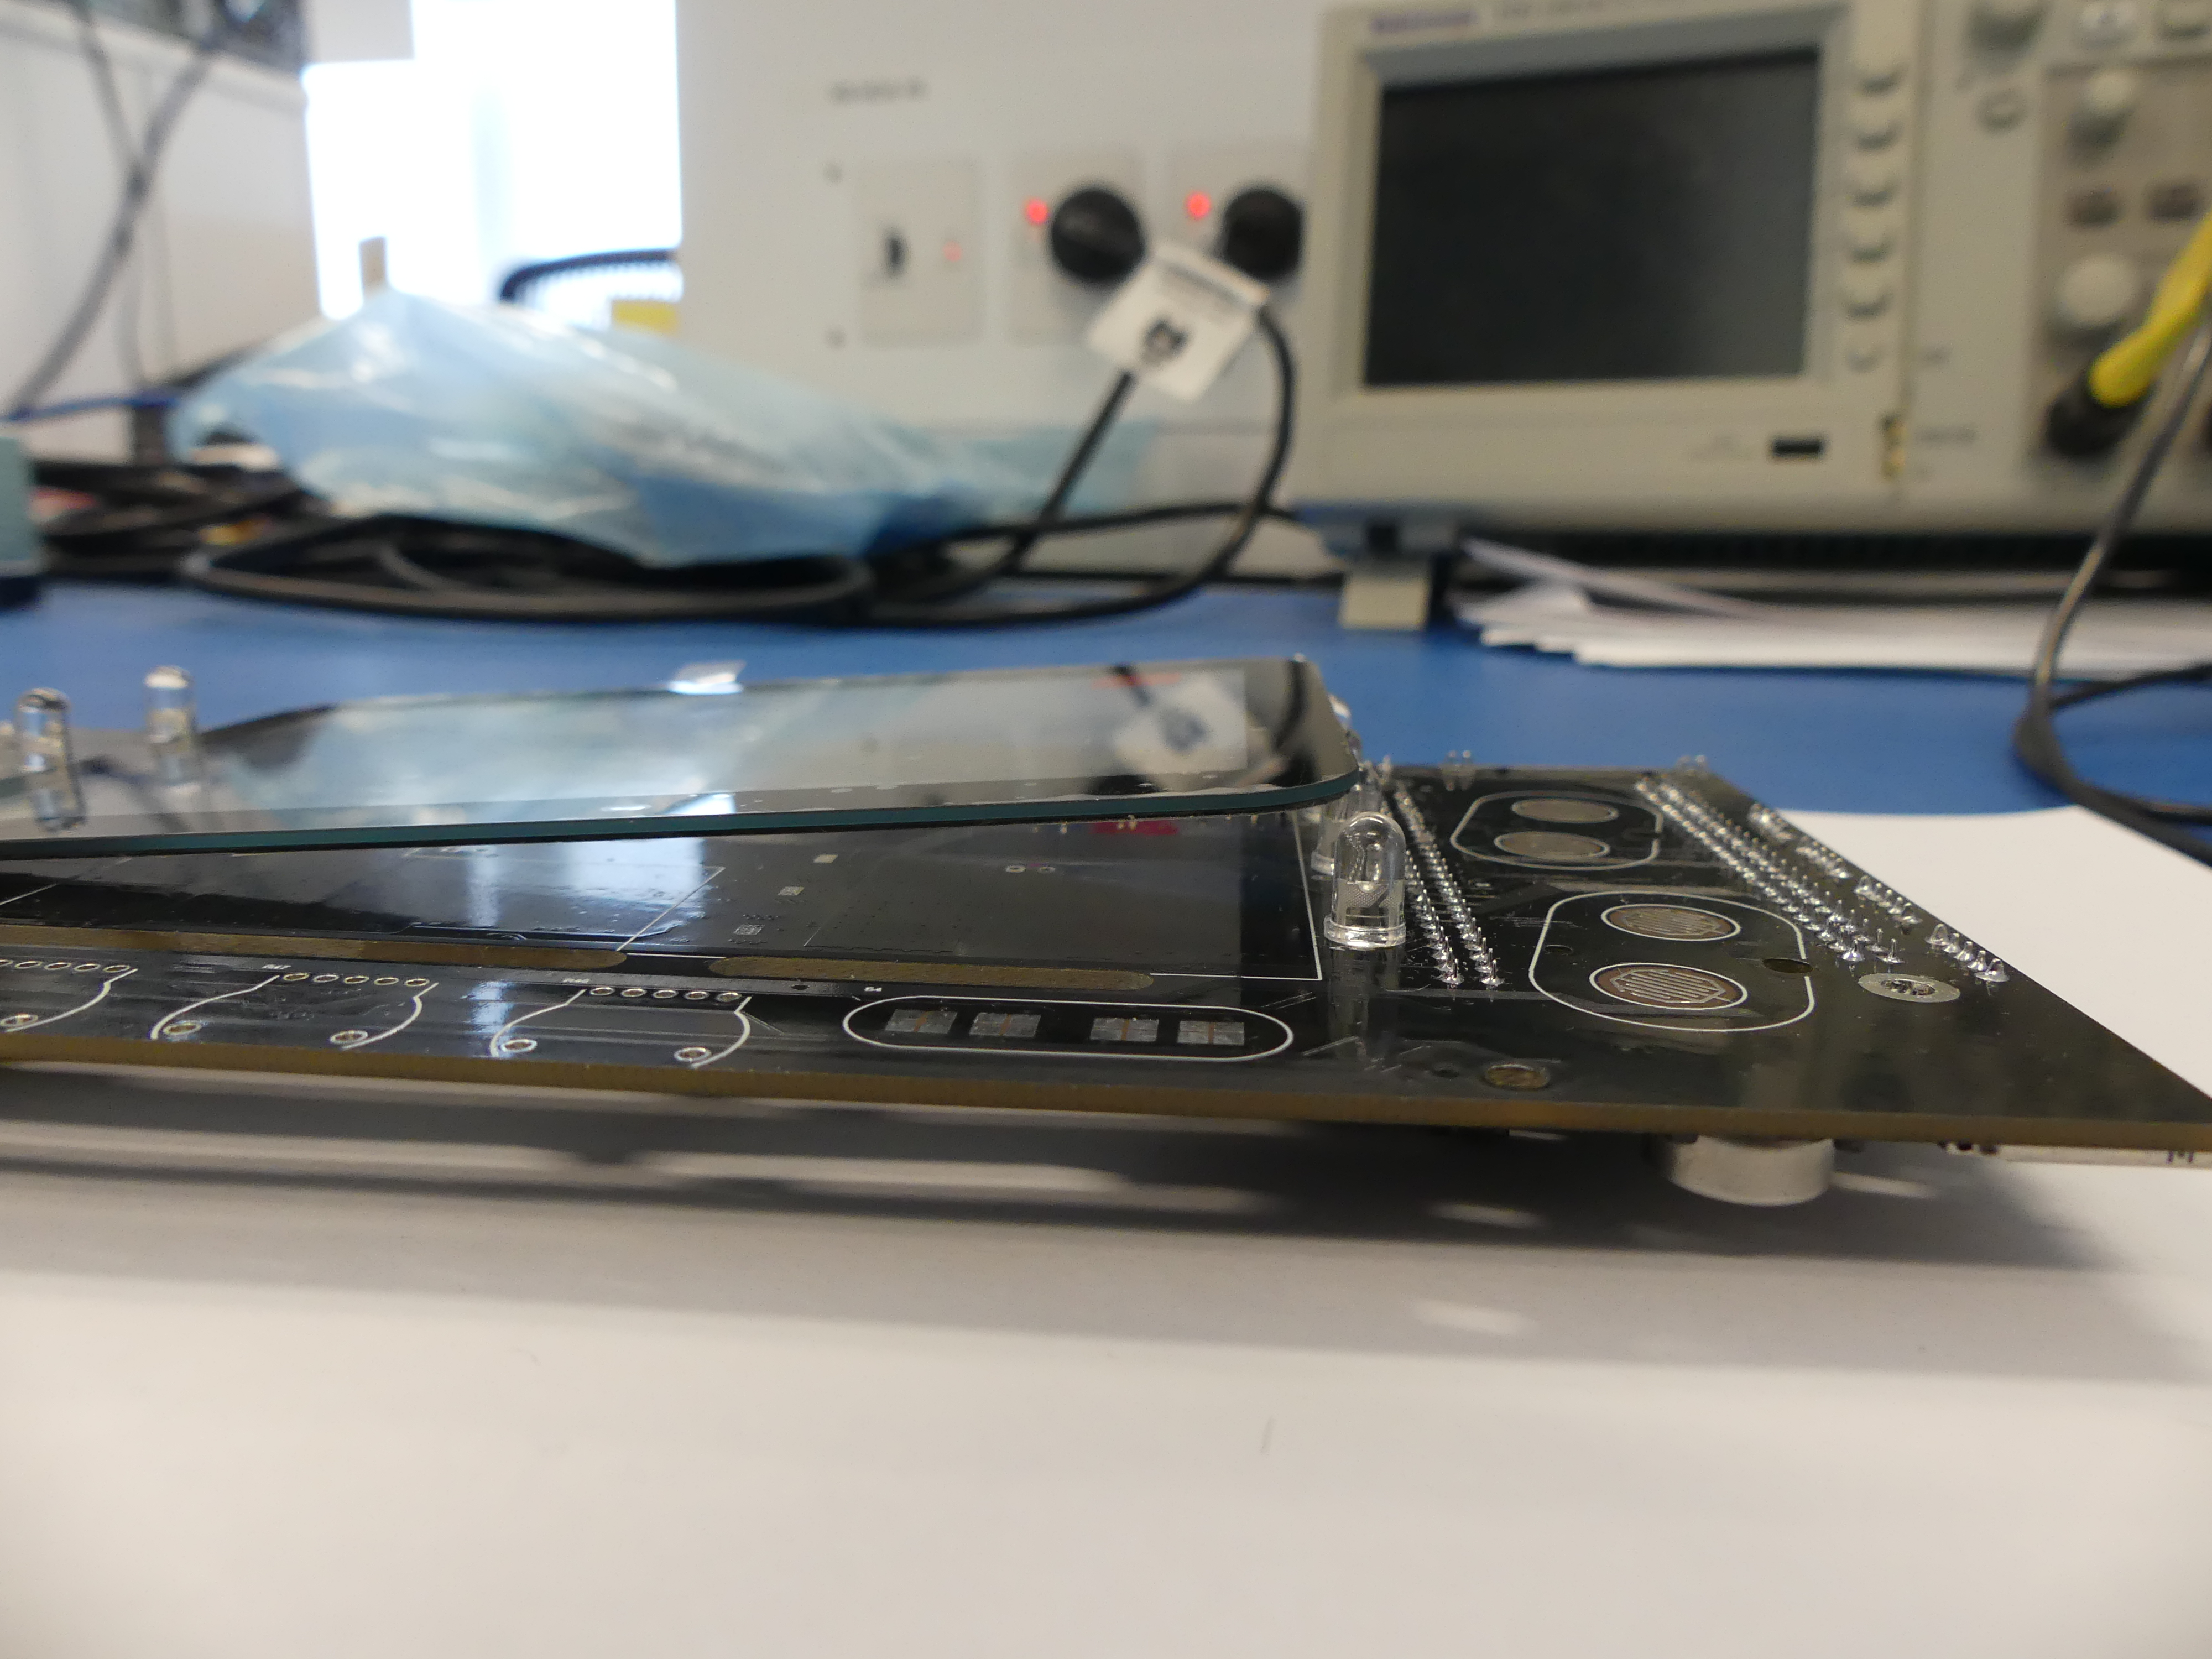
\includegraphics[width=.3\linewidth]{pics/MEGAphone_PCB_r1_LED3}
\end{center} 
\caption{Close up showing position of LED on front face of PCB. Screen cannot fit between them. \\}
\label{MEGAphone_PCB_r1_LED}
\end{figure}

\begin{figure} \begin{center}
\includegraphics[width=.3\linewidth]{pics/MEGAphone_PCB_r1_U9}
\end{center} 
\caption{Close up of U9 which didn't fit its footprint and had to be modified to fit. \\}
\label{MEGAphone_PCB_r1_U9}
\end{figure}

\begin{figure} \begin{center}
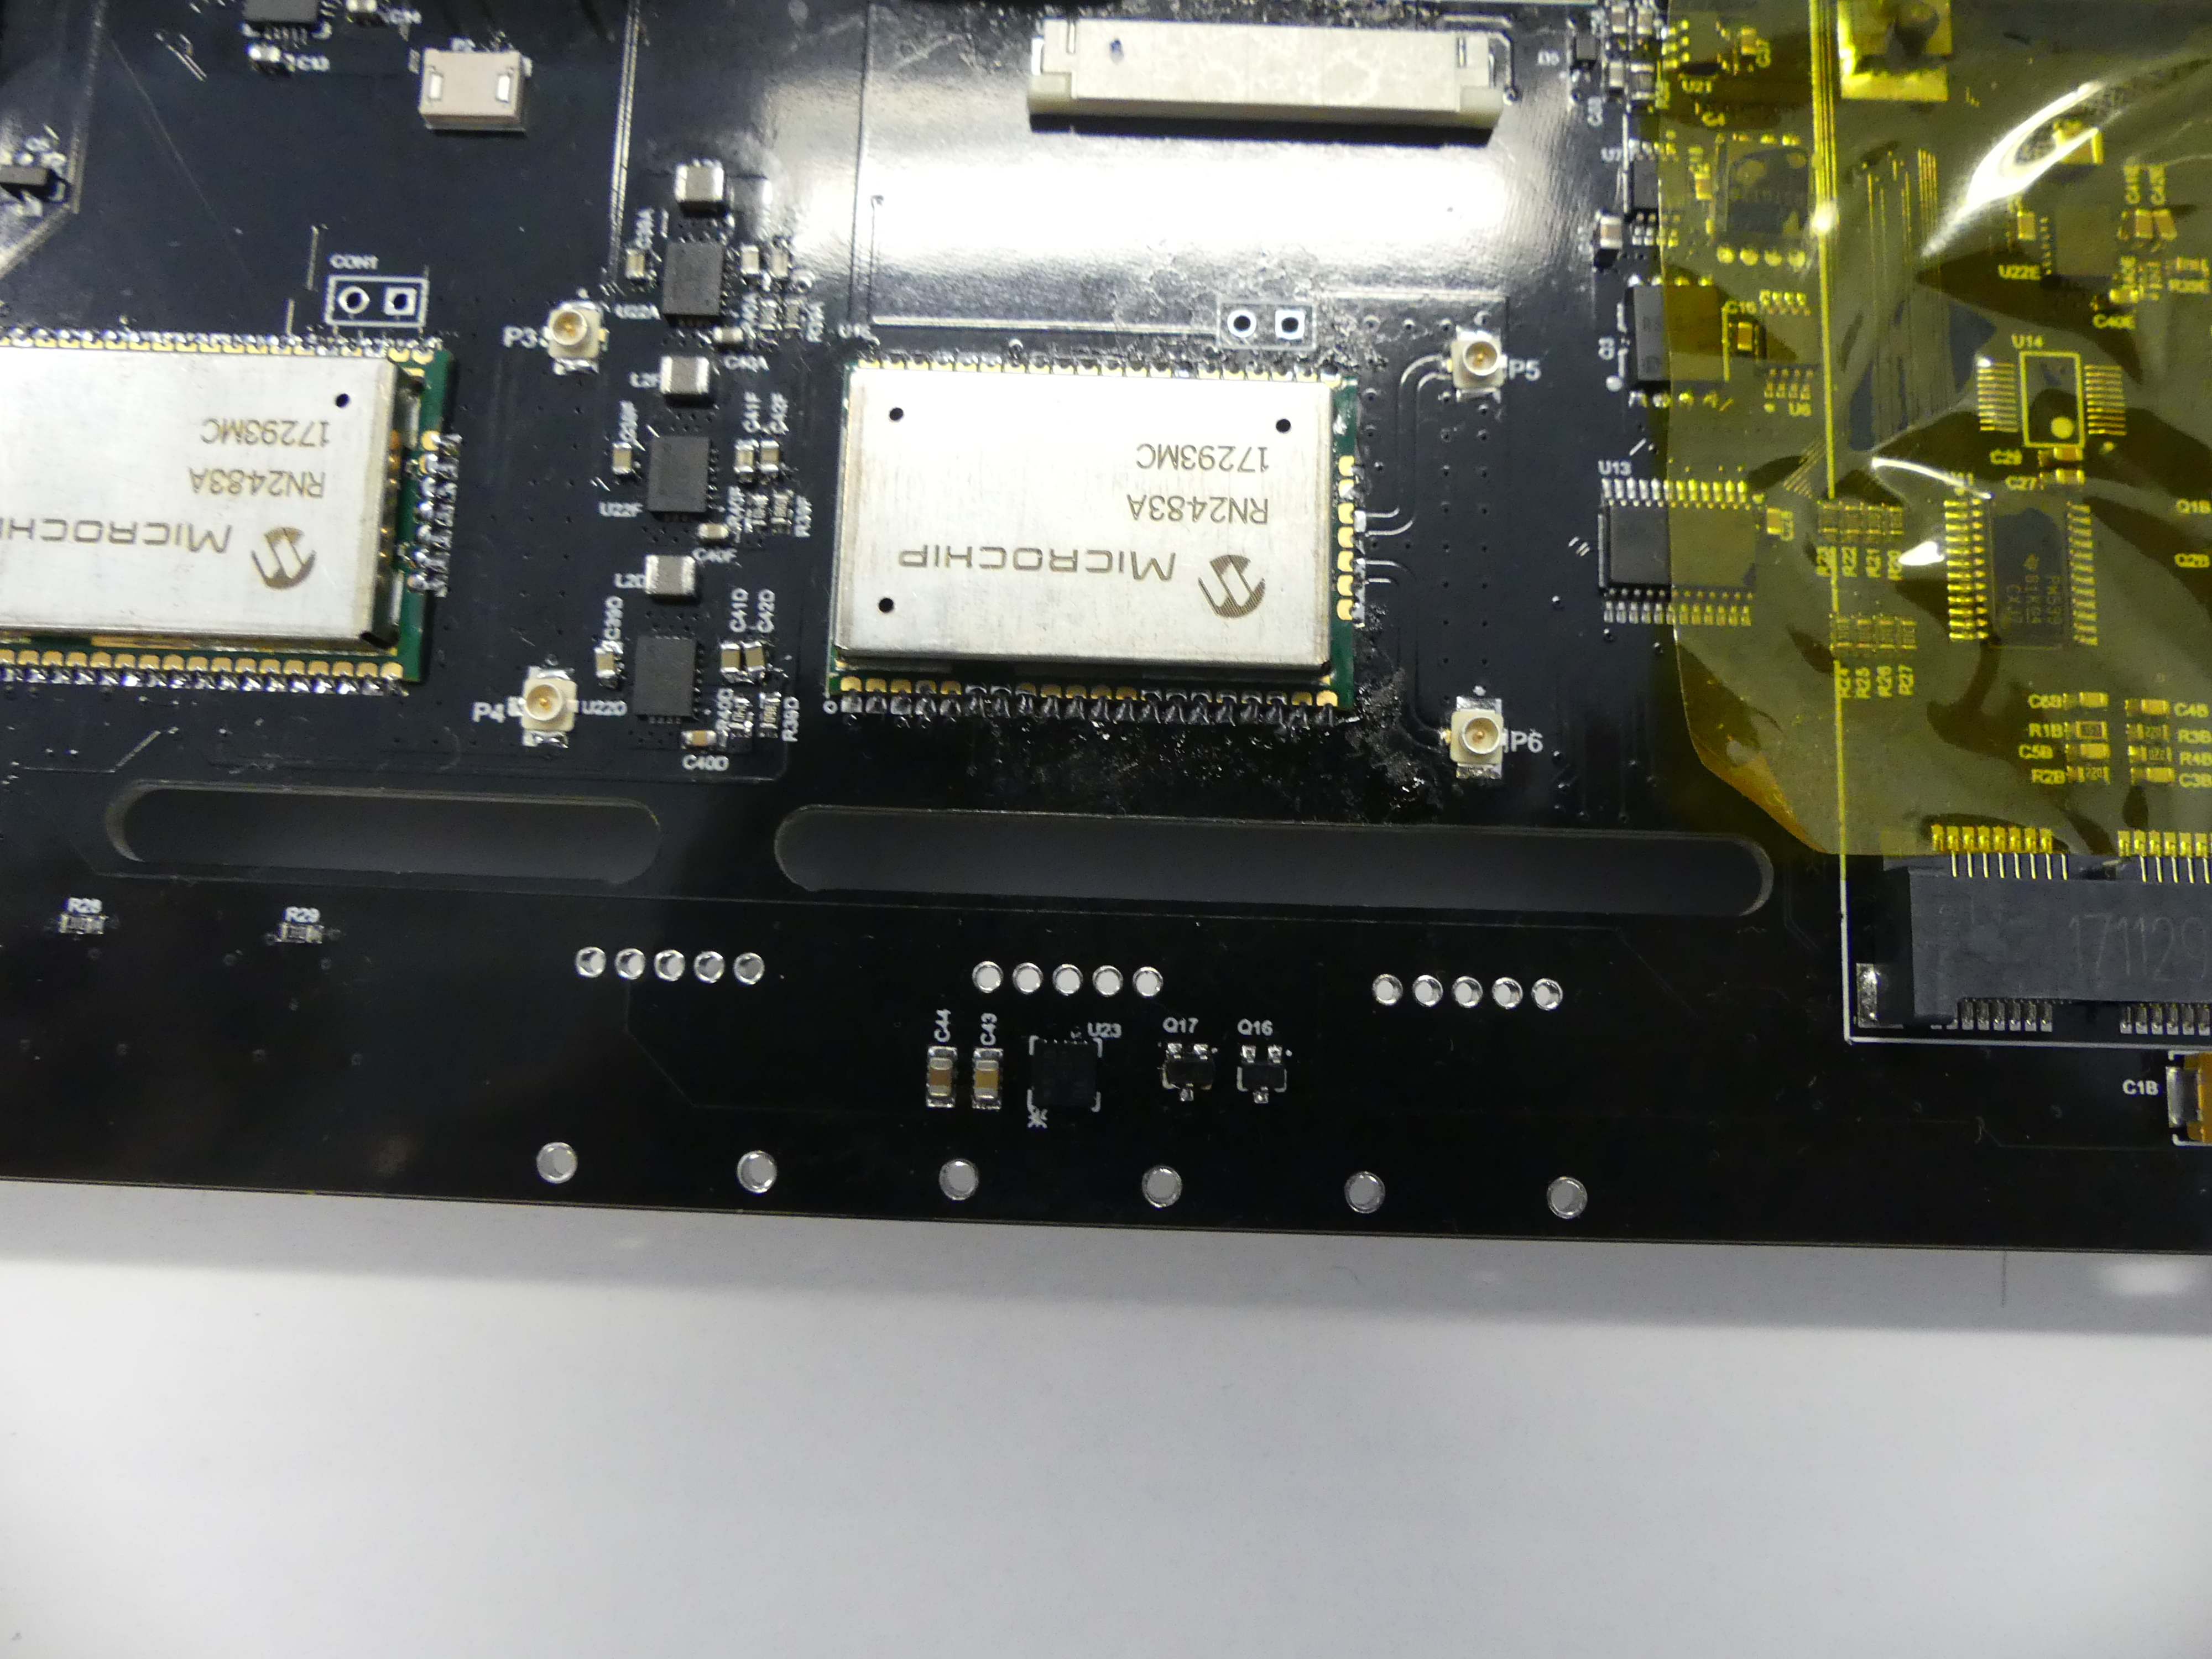
\includegraphics[width=.3\linewidth]{pics/MEGAphone_PCB_r1_R48_R47_R46}
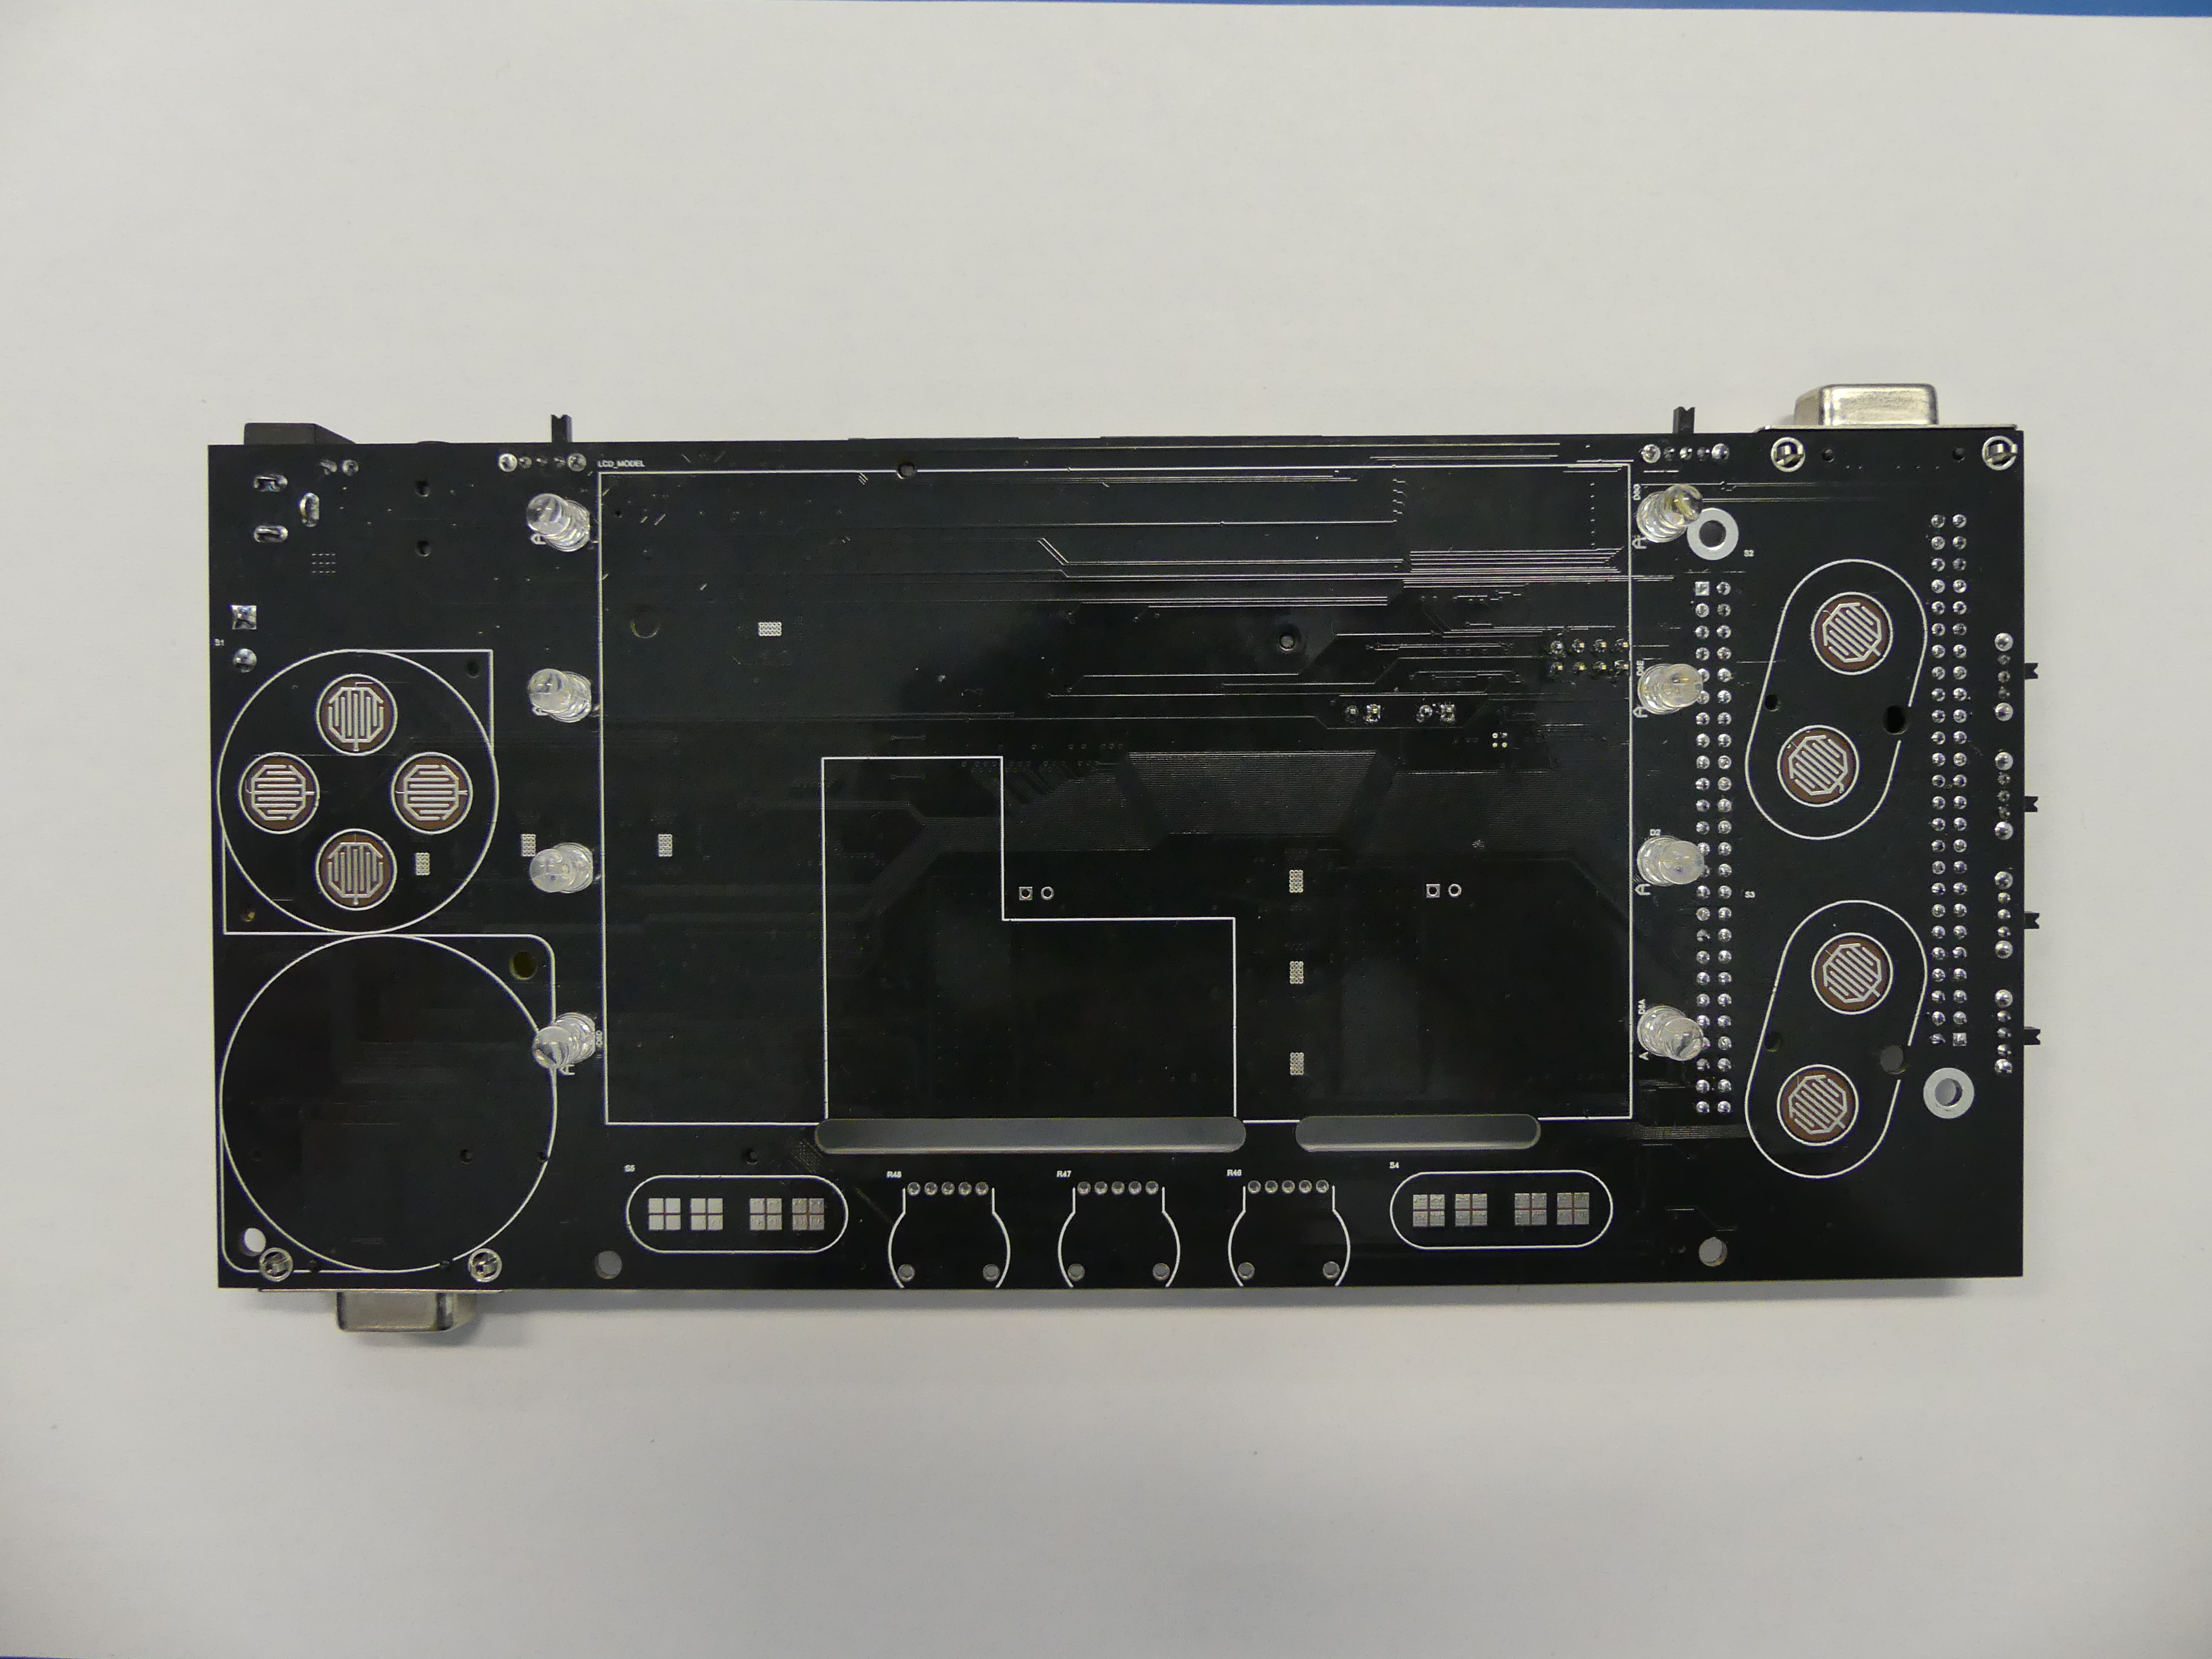
\includegraphics[width=.3\linewidth]{pics/MEGAphone_PCB_r1_populated_front}
\end{center} 
\caption{Close up of missing thumb wheels for volume control, R46, R47 and R48. \\}
\label{MEGAphone_PCB_r1_R49_R48_R47}
\end{figure}

\textbf{Things that need to be tested}
\begin{enumerate}
\item U1A and U1B, might not have enough clearance to fit the cellular modems in place due to components mounted on PCB in this area. 4G modem component to be used to test if it fits. Components within U1A and U1B footprint may need to be relocated if the 4G modem doesn't fit. In particular, the components J1A and J1B may need to be lower profile connectors such as a SIM card connector without the microSD slot above it, which it currently has on both J1A and J1B. Shown in figure \ref{MEGAphone_PCB_r1_U1A_clearance} \\
\end{enumerate}

\begin{figure} \begin{center}
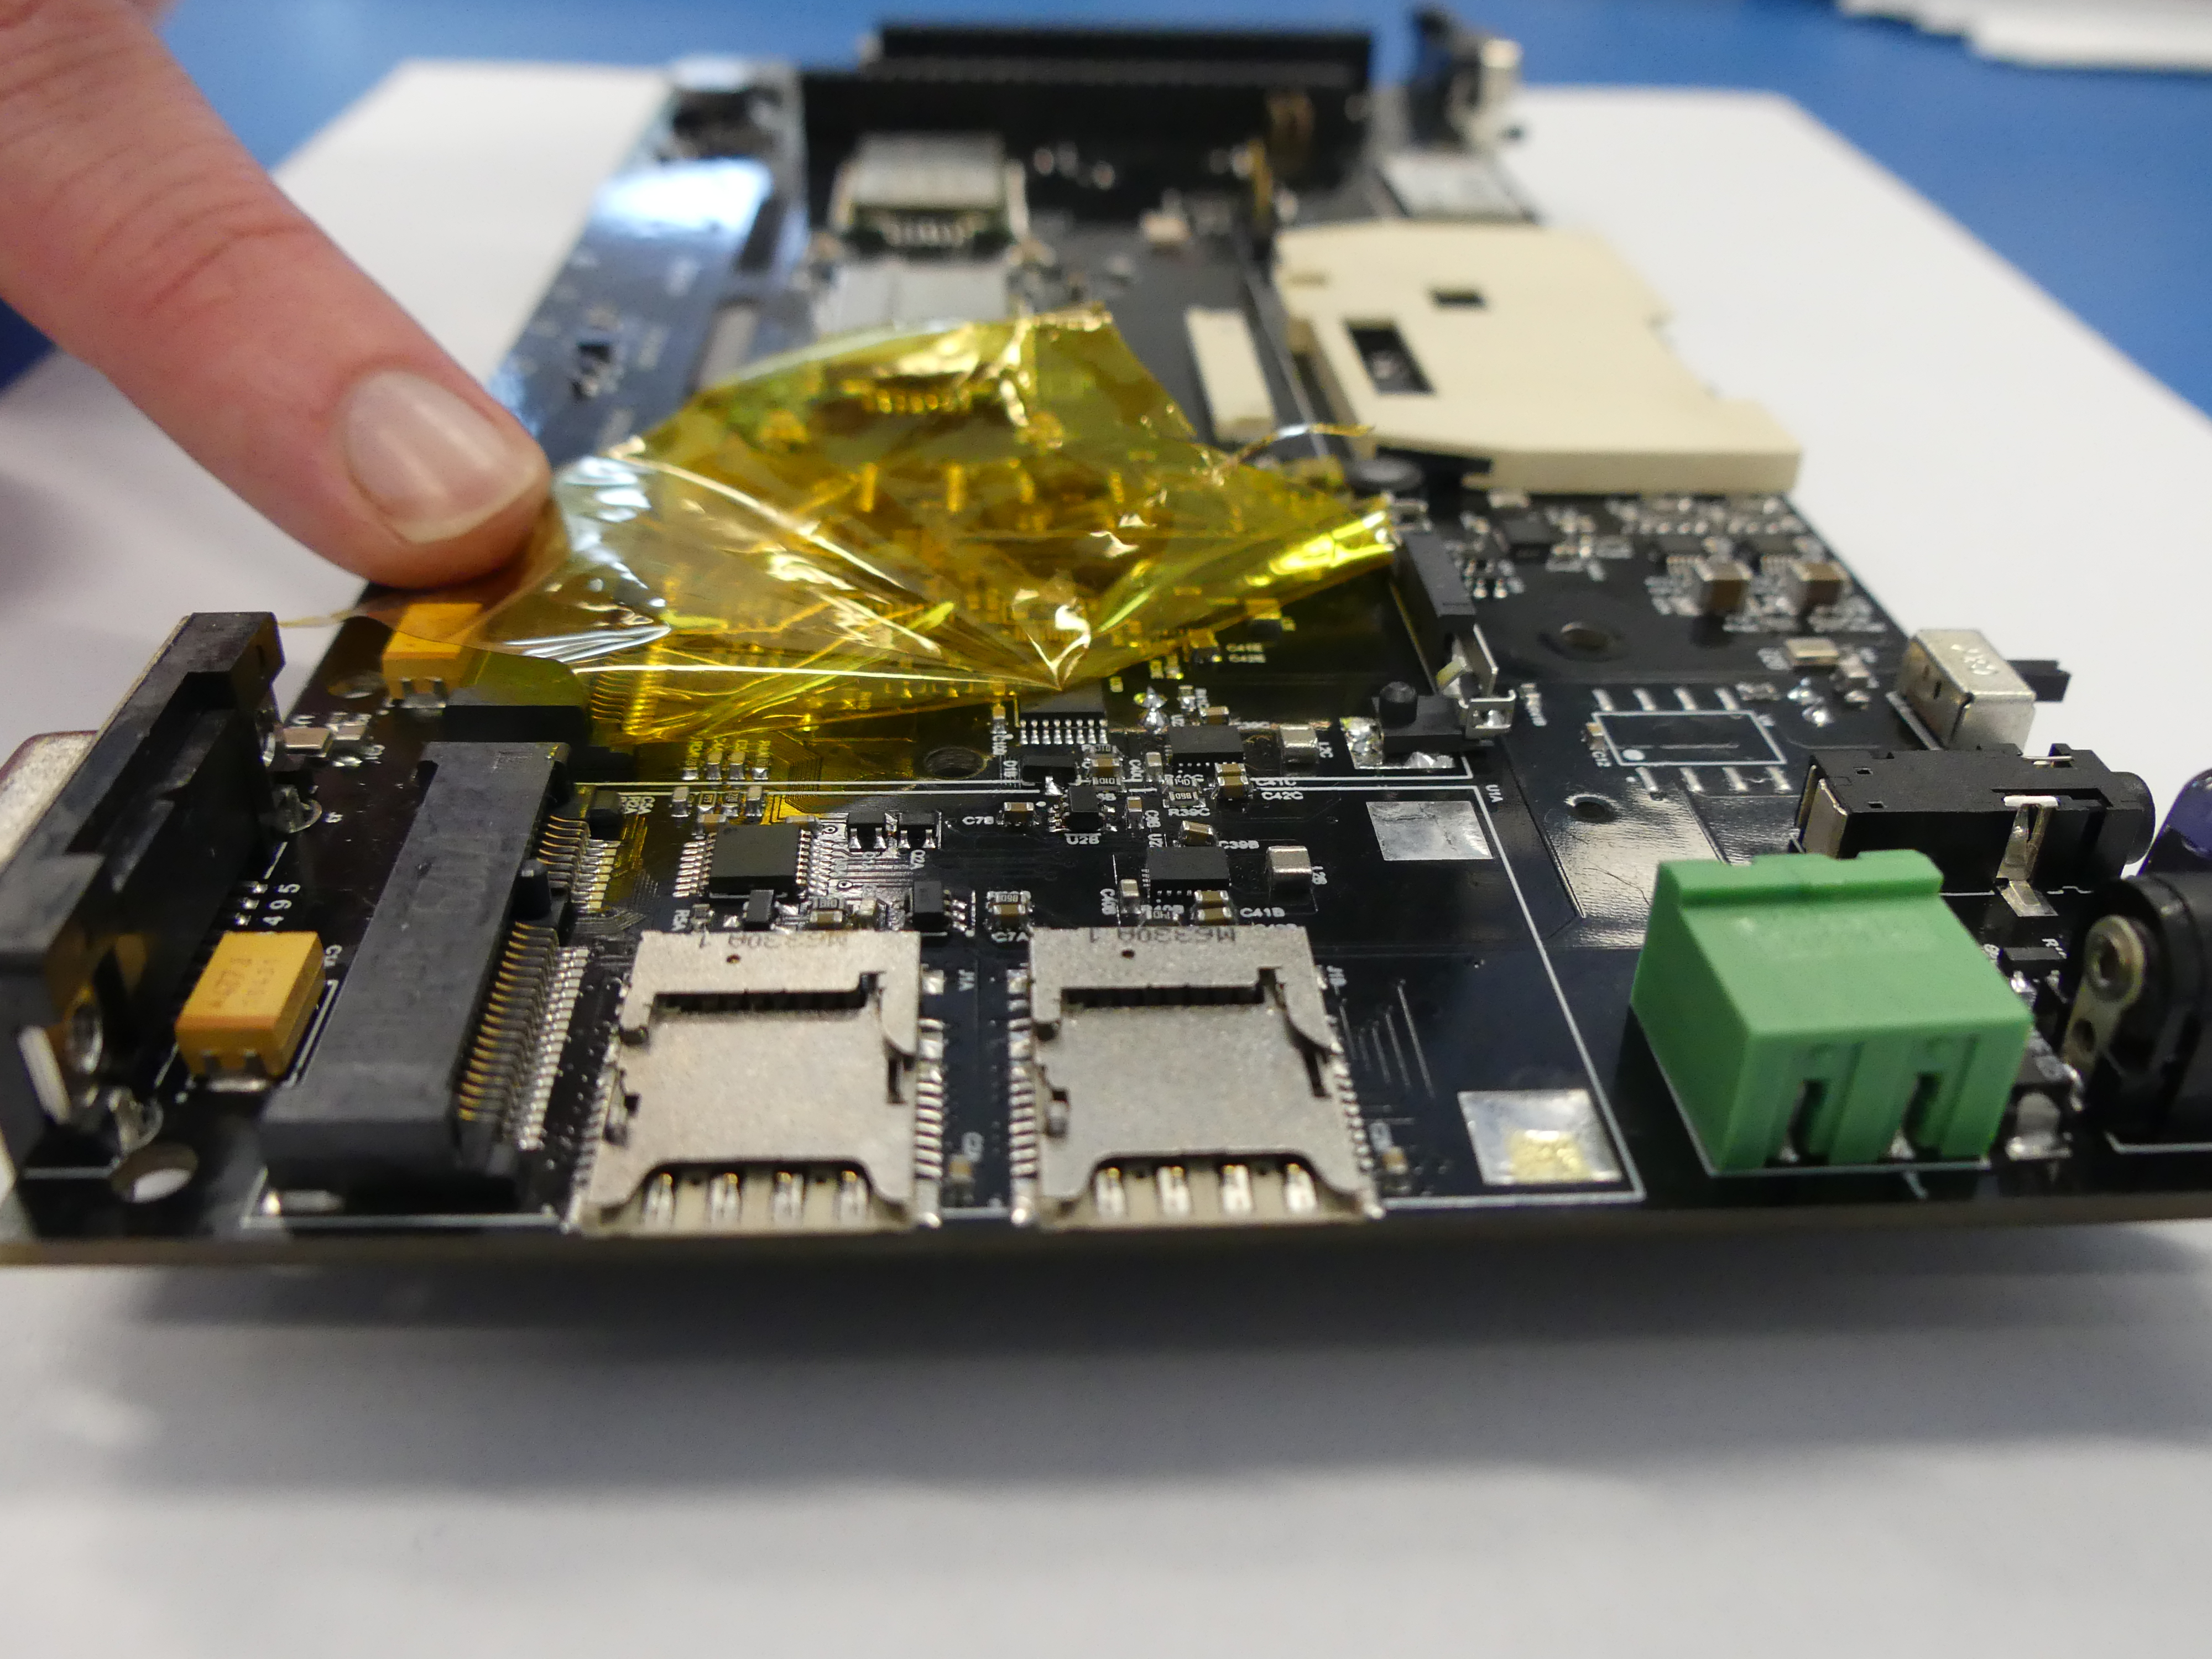
\includegraphics[width=.3\linewidth]{pics/MEGAphone_PCB_r1_U1A_clearance1}
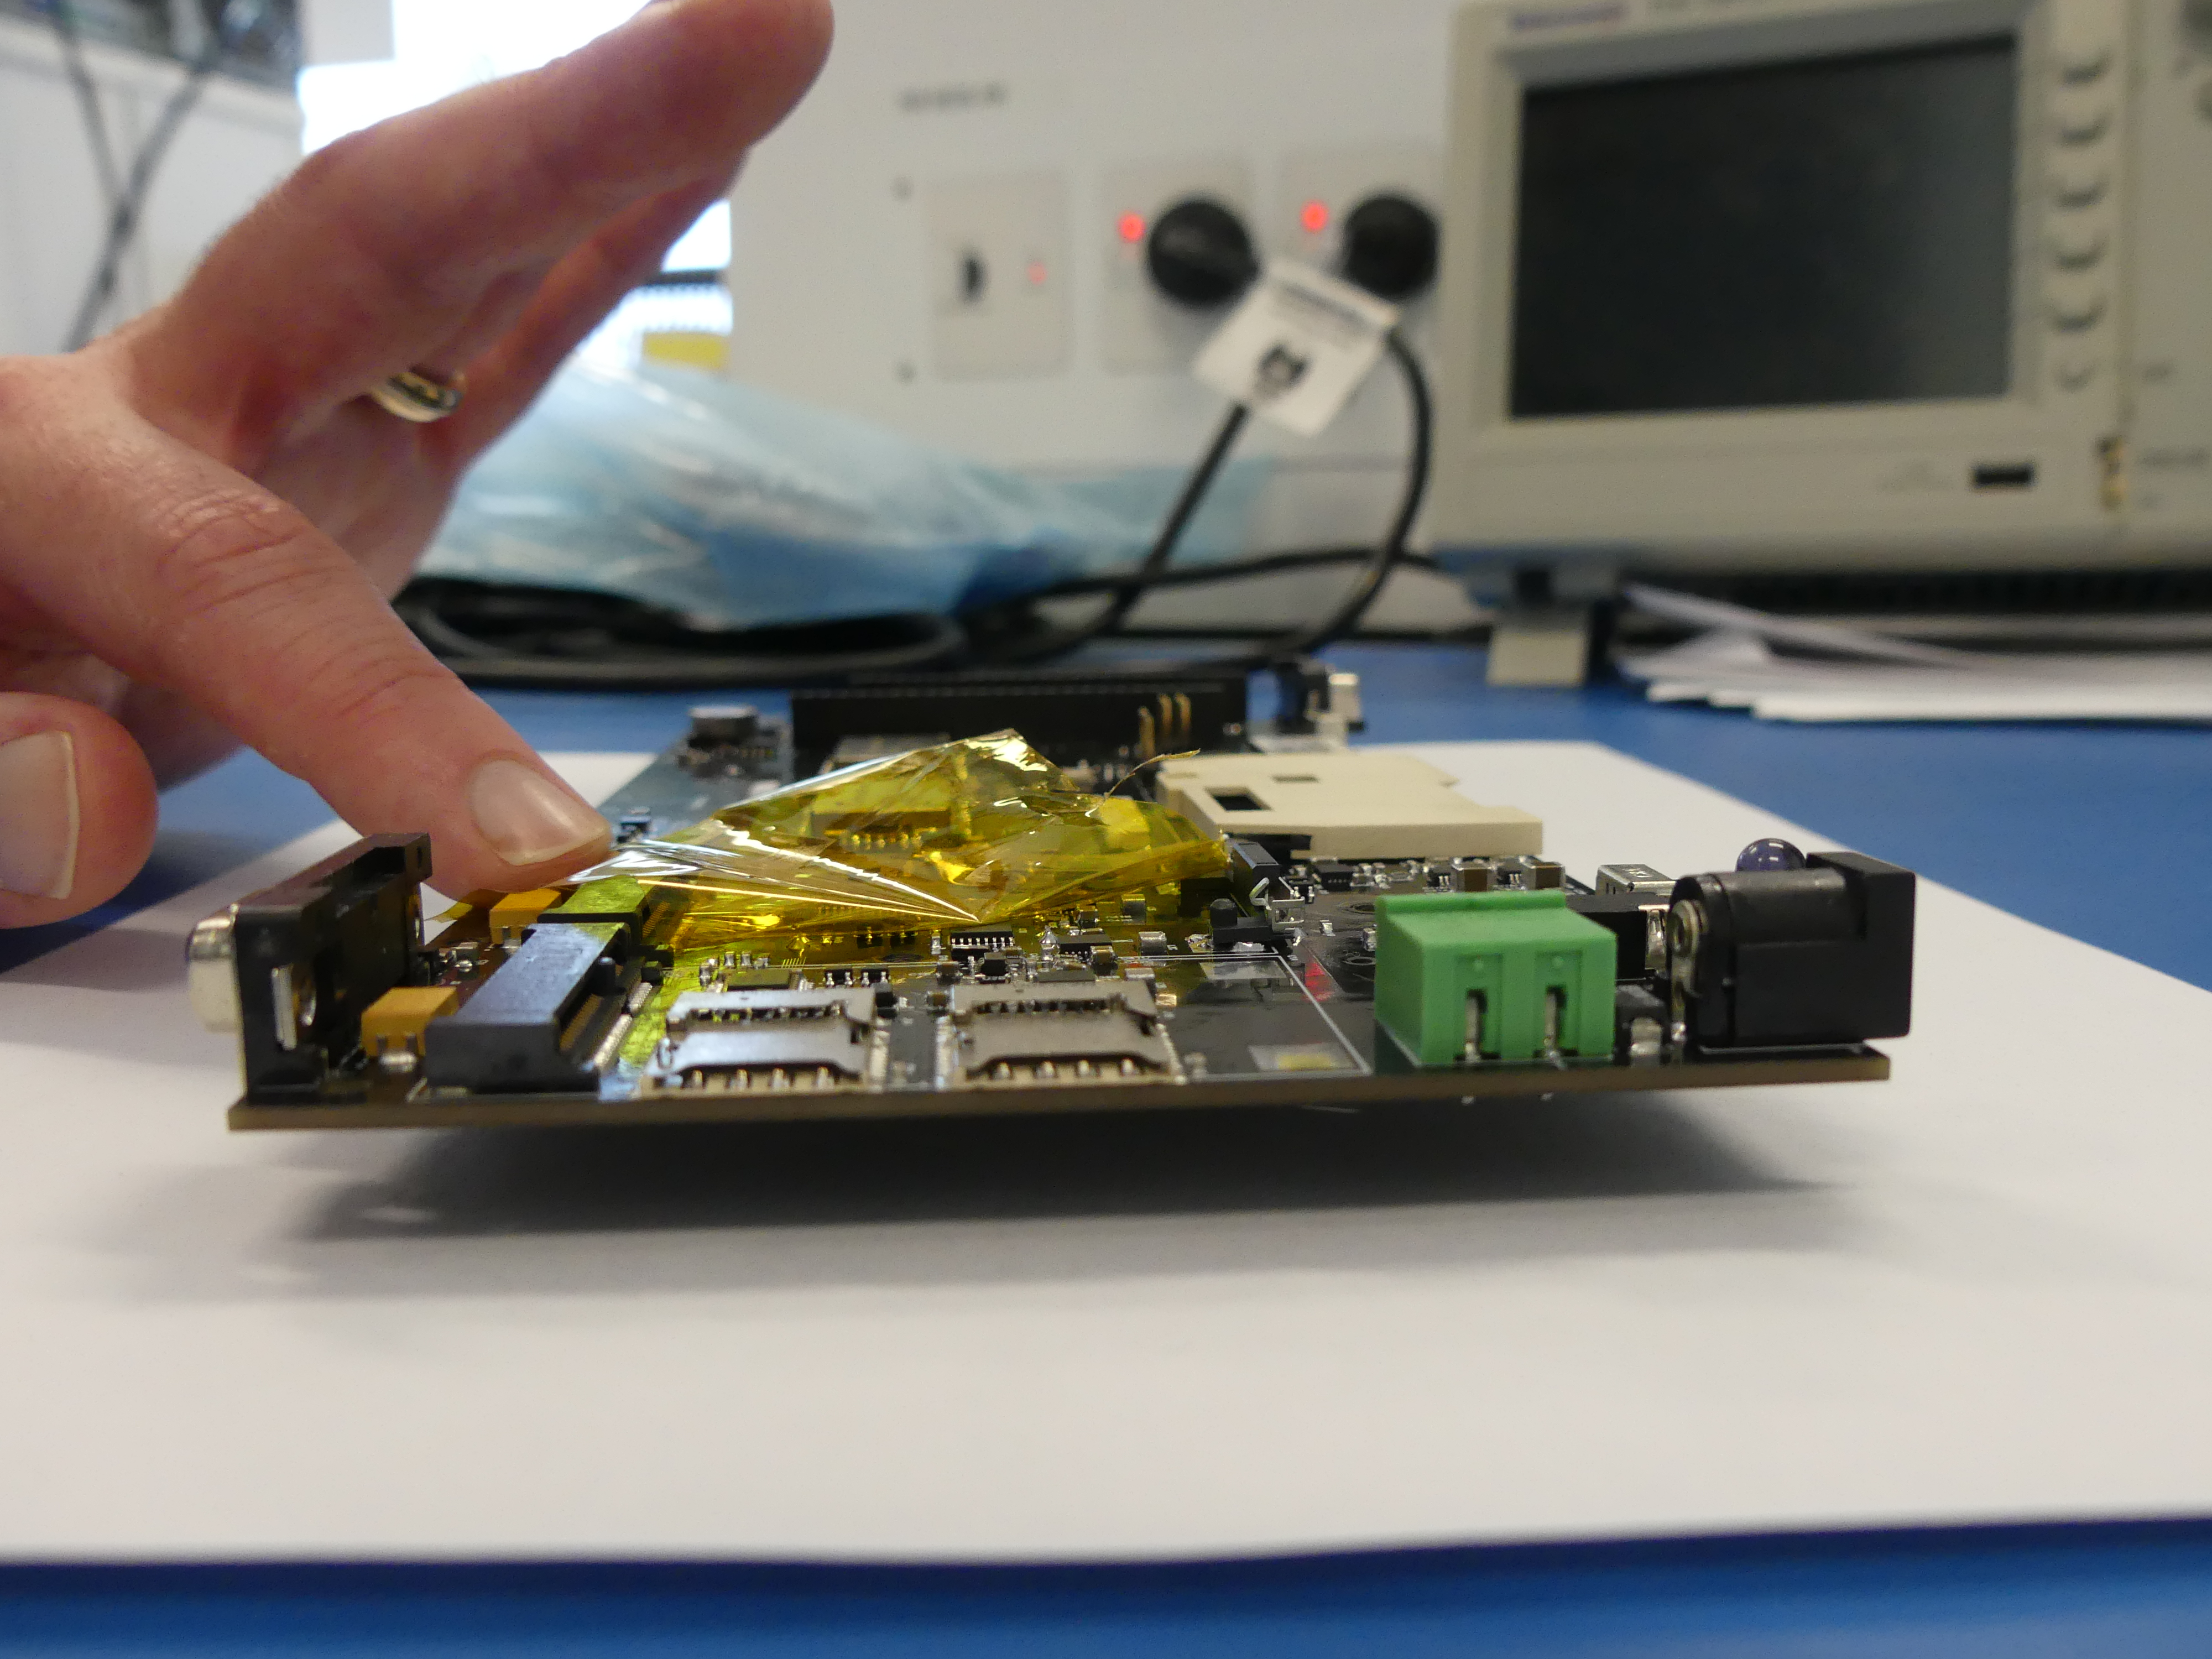
\includegraphics[width=.3\linewidth]{pics/MEGAphone_PCB_r1_U1A_clearance2}
\end{center} 
\caption{Close up of clearance above U1A and U1B footprints, a cellular modem needs to be inserted in this space. \\}
\label{MEGAphone_PCB_r1_U1A_clearance}
\end{figure}


\textbf{Components or functions which cannot be tested currently}
\begin{enumerate}
\item Microphone audio.
\item Thumb wheels for volume control, R48, R47 and R46.
\item 2nd PCIe modem slot, U1A.
\item 2nd SIM card slot, associated with the 2nd modem, U1A, mentioned above.
\item The ribbon cable connections between U25, P2 and the screen cannot be fully tested with the screen in position but a partial test with the screen offset should be possible.
\item Speaker currently not installed but parts and component are present in lab. \\
\end{enumerate}

\textbf{Noteworthy feature}
\begin{enumerate}
\item Installation of insulating tape covering components within the U1A and U1B footprints. This is to provide insulation between conductive part of components and the modem which will be inserted above them, seen in figure \ref{MEGAphone_PCB_r1_U1A_clearance} and \ref{MEGAphone_PCB_r1_U14}. \\
\end{enumerate}


\subsection{Software}



%----------------------------------------------------------------------------------------
%----------------------------------------------------------------------------------------
\section{MEGA65 Desktop Computer Form Factor}
This section looks at the current state of the MEGA65 Desktop form-factor. The Desktop form-factor's physical development is being overseen by M.E.G.A. in Germany. The physical development refers to the electronics hardware, case and keyboard. It still uses the same FPGA-based core, developed by Dr Gardner-Stephens, as the MEGAphone. Following a discussion the Detlef in Germany, who is overseeing the development of the MEGA65 Desktop, the following state of the MEGA65 Desktop hardware was elicited. 

The MEGA65 Desktop is currently in a "pre-series" stage, the machines are roughly 95\% complete and have been created in their current state so they can be tested in a real-life environment. 

\subsection{Hardware}


\subsection{Case}
The current case has had a few modifications from the original design, which was based on the Commodore 65 case. It has a new appearance with a original case design which has been described as "cleaner". The new case also has some major changes around the port at the back of the computer and some minor changes to the trapdoor on the bottom as well as some additions for ventilation. These design changes to the new case where carried out by Hintsteiner in Austria.

The MEGA65 Desktop is planned for a pre-production run of 20 machines using the new case design. This run will use vacuum moulds for the cases to reduce costs but the vacuum mould process has some drawbacks: 
\begin{enumerate}
\item The mould will only only be bale to create 20 cases before it has to be replaced.
\item The colour of the plastic forming the case slightly changes between cases.
\item Some parts of the case need to be manually fixed after the vacuum mould adding costs and the need to paint sections of the case.
\end{enumerate}

*PIC OF NEW CASE TO COME FROM DETLEF*

\subsection{Keyboard}
The keyboard for the MEGA65 Desktop is being produced by GMK, a German company. It features Cherry MX mechanical switches and 2 embedded metal plates, intended to provide very high stability. There are 2 LEDs for the lock keys, capslock and numlock and 4 RGB LEDs for power and floppy activity indicators, these are all powered by a custom-made communication bus. The keyboard also has a CPLD-based controller in place of the more widely used ARM7 microcontroller, this was done intentional to avoid "having more intelligence inside the keyboard than inside the computer".

Detlef has ordered 25 keyboards for the pre-production run, this was intentionally more than the 20 cases being produced, as mentioned above. It will provide for 5 case-less machines to use as spare-parts. It is expected that the keyboards will be in a finished state and require no more design work 

\subsection{PCB}
The PCB provides the interface between the FPGA architecture and the physical circuitry required for such features as the LEDs, I/O ports, speakers and keyboard. The design of the PCB for the MEGA65 Desktop version is being carried out by Antii Lukats at Trenz Elektronik. Currently Lukats is working on the 'r2' version of the PCB and it should be finished in early April, 2019. From there a pre-production run of 25 will be manufactured and then populated with components, before being send to Detlef. 

During the design of the PCB, a challenge arose from the need to combine modern components with much older components such as the floppy disk connector and the 9-pin joystick port. This required a larger number of different voltage levels to power the components than a purely modern component machine. 

\subsection{Other Components}
To make a finished product the MEGA65 will need more than the computer its self, there also needs to be considerations and preparations made for such things as the box, manual, silica gel for packing, warning and warranty paperwork and CE certification paperwork. To complete the computer itself also requires some extra items such as serial number stickers, warranty seals/stickers, type signs, power supply units, screws, SD card, floppy drives and cables.